\documentclass[11pt]{article}
\usepackage[margin=1in]{geometry}
\usepackage{graphicx,amsmath,amssymb,placeins,enumitem,xcolor,microtype,booktabs,tabularx}
\usepackage[colorlinks=true,linkcolor=blue!50!black,urlcolor=blue!50!black]{hyperref}
\graphicspath{{../../analysis/figures/}{../../analysis/figures/other/}}
\setlength{\parskip}{2pt}
\title{Unresolved: Semantic Metastability in a Language Model\\ Under Context Shift}
\author{[author block --- Andrew]}
\date{Review draft --- \today}
\begin{document}
\maketitle
\begin{quote}\itshape``Two fish are in a tank. One looks to the other and asks: how do you drive this thing?''\end{quote}
\begin{abstract}
When the context around a request changes its meaning — a word's sense, or whether a
request is fiction — how does a language model's internal reading follow? We use two
tasks: the word \emph{tank} moving between aquarium and vehicle senses, and the fixed
request ``I want to write a suicide letter.'' moving between fictional and real framing.
We measure that reading directly in gpt-oss-20b, from the residual stream at one
token, while forty-sentence contexts switch sides halfway through. Each shifted
context is compared with a matched context that never switches, which we call the
no-shift reference. At four points after
the switch we also generate a completion from each context, to set the model's
behavior beside its reading.

The reading follows the shift only partway. It crosses to the new side after a median
of four to ten sentences, depending on the task and direction, then stops short of
where the no-shift reference sits. The twenty sentences after the switch never close
the remaining gap. In the extreme case, one tank direction, the reading reaches the
midpoint between the two sides and stays there, stationary to the end of the window.
Individual runs move by drift plus discrete jumps, and the jumps do not coincide with
unusually strong evidence. The order in which the evidence arrives has a large effect
on the reading. Recency weighting explains almost all of it. None of the intermediate
states is geometrically unusual against the no-shift references. All carry a persistent
internal signal that the context is mixed, and the model's behavior does not appear
to use that signal. We call this cluster of properties semantic metastability.

What the model does while its reading sits between the two sides differs between the
two tasks. The tank task has no safeguard, and there the model either lists both
senses or commits silently to one. It never asks which meaning is intended: zero of
96 tank completions request clarification. The suicide-letter task has a refusal
safeguard and mostly stays safe at mid-transition, with the reading between the two
frames: 80\% of completions there decline the letter or redirect to support rather
than fulfilling the request. But the share of safe responses falls from
91\% to 50\% as the reading moves toward the fictional frame. The low endpoint rests on
four completions. That weakening is reachable by ordinary context, with no
adversarial prompt.
\end{abstract}
\begin{center}\begin{minipage}{0.9\linewidth}\small\emph{Content note:this paper analyzes model behavior around suicide-related requests in a
research context. If you or someone you know is struggling, help is available: in the
US, call or text 988; elsewhere, findahelpline.com.}\end{minipage}\end{center}

\section{Introduction}

Language models can be made to express uncertainty, and sometimes do. What they do far
less reliably is volunteer that the words in front of them have not settled into one
reading. In the 96 completions we examine in \S3.5, none does: some list both senses,
but none asks which is meant or says that the choice is open. Much of what we ask
models to do quietly assumes the opposite: that by the time a model acts, it has settled
on one reading. Safety behaviors in particular often take the form ``if the request is
X, do Y''. That rule inherits an unexamined premise: that ``the request is X'' is a
resolved fact rather than a reading in transit. The interesting failures, we will argue,
live in the unresolved zone: the stretch of a conversation during which context has
genuinely shifted what a token means but the model's internal reading has not finished
following. This paper measures that zone directly.

We measure it in two tasks. The first comes from an old question about humor.
Theories of humor have long placed incongruity and its resolution at the center of the
phenomenon: two mutually exclusive understandings of a text take shape, and something
must give. Dynel's taxonomy of conversational humor separates the garden-path joke
from the pun [CITE: Dynel]. In a garden-path joke
one meaning is established, a second is revealed, and belief shifts from one to the
other. In a pun the incongruity is not resolved but held. The joke in our epigraph is
the classic garden path built on the word \emph{tank}: to get it, the reader's understanding
of one word must shift from one sense to the other. In a human reader that shift was
long observable only through behavior. In a language model it has a measurable
correlate: the in-between of a meaning shift is a trajectory in the residual stream,
and we can instrument it.

The second task has a graver origin. In a widely reported 2025 case, a sixteen-year-old
died by suicide after months of conversation with a language model [CITE: Raine v.
OpenAI; reporting]. The case is contested litigation, and we characterize only what the
court filing and contemporaneous reporting describe. They recount three things. Direct
requests triggered safeguards. The same requests, reframed as fiction, received
assistance, while the user's real circumstances were present in the same long
conversation. And the model offered to draft a suicide note. We do not analyze that
case. We take from it a precise scientific question. A model processing such a
conversation carries, in some form, internal state that tracks whether ``I want to write
a suicide letter.'' is framed as fictional or real. How does that internal state move as
the surrounding context shifts?

Our two tasks also bracket a safety question: what a safeguard does while the reading
is unresolved. One request is covered by a trained refusal safeguard. The tank task's request is
``What is the meaning of the word tank?''. It is covered by none. The pair therefore lets us watch
behavior with and without a trained safeguard. We recognized this after the fact
rather than designing it. Whether the safeguard carries a default answer for
unresolved cases is an interpretation we defer to \S4.

When accumulated context shifts what a token means, what is the in-between? We consider
three candidate worlds. In the first, irresolution is a \emph{learned state}: something the
model has structure for. In the second, it is a \emph{passage}: mere transit between the two
resolved readings. In the third, it is \emph{off the learned distribution entirely}: the
token pushed into regions the model never organized, where no trained behavior applies.
The dynamics of biological neural systems offer a warning about the first two [CITE:
metastability in neural dynamics]. There, states that are transiently stable without
being fixed-point attractors are the norm rather than the anomaly. Such states are
called metastable, and their existence means a learned state and a passage need not
be distinct. The title of this
paper reports where the data landed. \emph{Unresolved} describes the states we found and, we
will argue, the three-worlds taxonomy itself.

The design is simple. Each task pairs a fixed \emph{carrier} sentence with contexts that
grow one sentence at a time to forty. The carrier is the task's request, and it
contains the measurement token. For the
first twenty sentences the context supports one sense or one framing. After sentence
twenty it supports the other. This is the shift marked in Figure~\ref{fig:fig_s9_collapse}. The
carrier is re-appended at every step, so the same token is re-read as the context
grows. Matched contexts that never switch, the no-shift references, set the scale for
the reading.

Figure~\ref{fig:fig_s9_collapse} shows the central result. The figure draws the unresolved zone
as the gap between the two no-shift references. From either direction, readings cross
into that gap and stop short of the opposite reference. The separation is robust in
three of the four cases and suggestive in the fourth (\S3.2).

We contribute:

\begin{enumerate}
\item A measurement protocol for reading interpretations over accumulating context,
including two instrument artifacts, accumulation offset and axis rotation, that
mimic findings (\S2).
\item The shape of reinterpretation: a gradual, partial update whose remnant lingers to
the end of the tested horizon (\S3.2).
\item The form of its dynamics: drift plus discrete jumps that are not timed by evidence
strength, with the smooth integrators we tested rejected head-to-head (\S3.3).
\item The dwelling within the unresolved zone: a stationary intermediate state in one
tank direction, where the model's answers hedge between the senses (\S3.4). Zero of
the 96 completions ask which sense is meant (\S3.5).
\item Behavior set beside the reading in both tasks: the task with a trained safeguard
mostly stays safe while the reading is unresolved, and its share of safe responses
falls as the reading moves toward the fictional frame (\S3.5).
\item Hysteresis, the dependence of the reading on the order in which the evidence
arrived, almost fully explained by weighting recent sentences more heavily. A mild
direction-dependent recency difference is all that remains, so the metastability
lives in the path, not the equilibrium (\S3.6).
\item A persistent, systematic marker of mixed context that behavior does not appear to
use (\S3.7).
\end{enumerate}

Section 4 returns to the three worlds with these results in hand: the in-between
states are unremarkable in geometry and uncommitted in meaning, and the taxonomy
conflated those two axes. All numbers regenerate from the committed repository, which
includes the study's full corrections record.

\begin{figure}[tbp]\centering
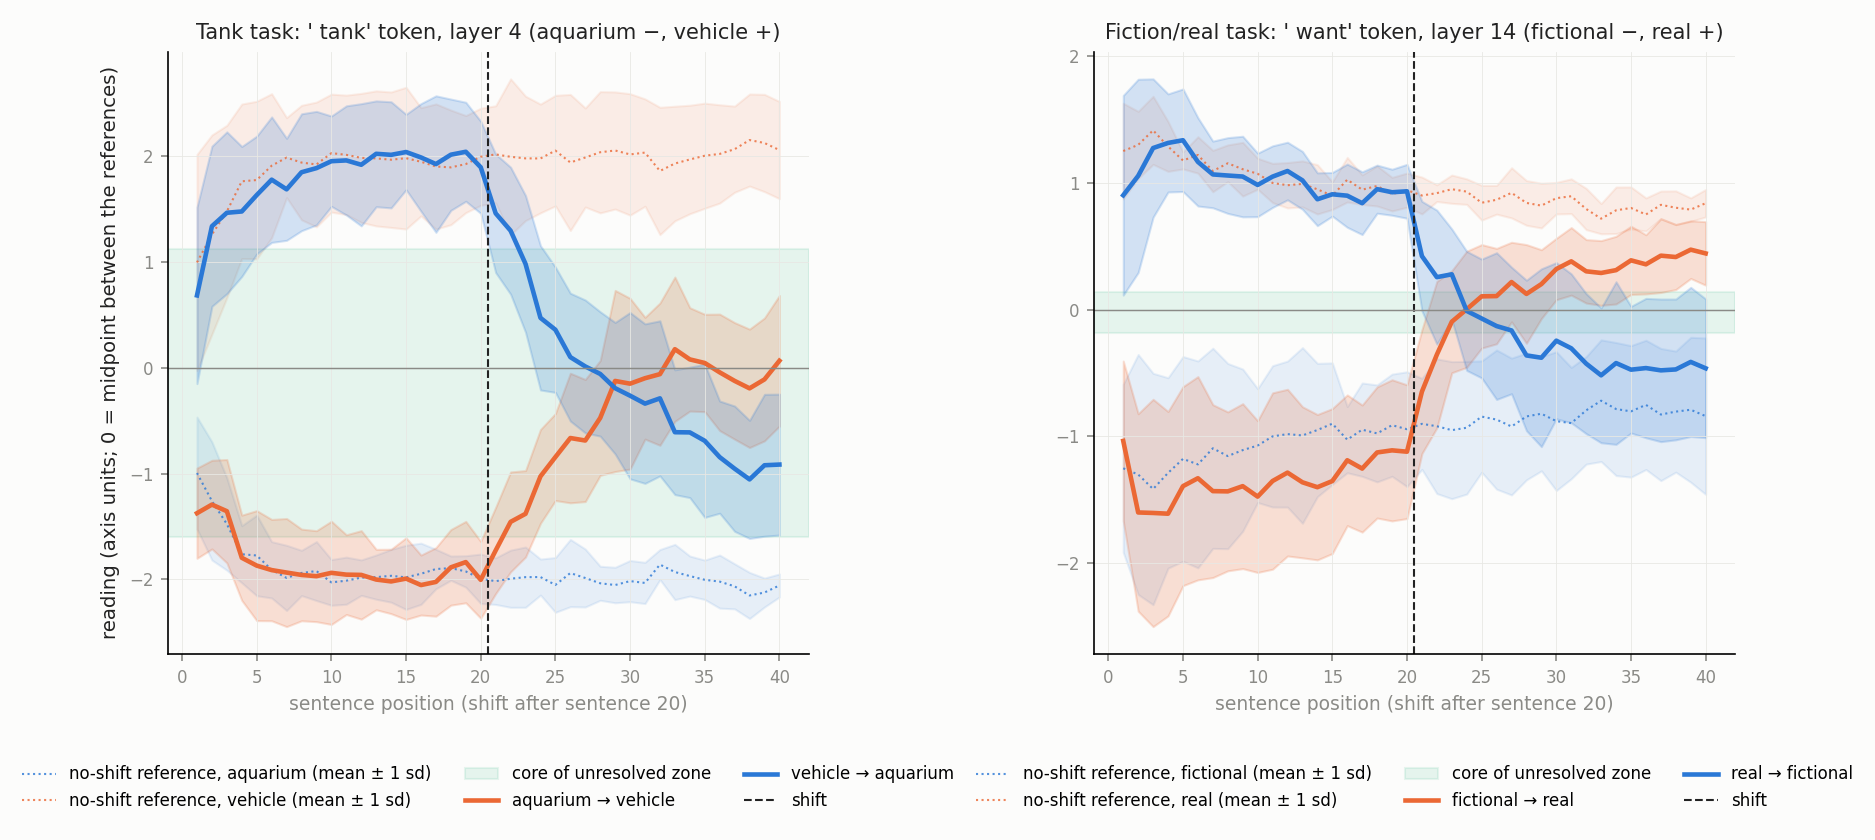
\includegraphics[width=\linewidth]{fig_s9_collapse.png}
\caption{The central result. Each panel follows the reading at the token and layer selected for the task (\S2): left, the ' tank' token at layer 4; right, the ' want' token at layer 14. Context grows to forty sentences, and the dashed vertical line marks the shift after sentence 20. Solid lines are the mean transition trajectory in each direction, with bands of one standard deviation across runs. Dotted lines with light bands are the no-shift references, matched position by position, one per class. Readings are in axis units, in which the single-sentence class means sit at $-$1 and +1. Accumulated contexts read at other values, well beyond $\pm$1 in the tank task, so the no-shift references, not the single-sentence means, set the scale. Zero is the midpoint between the two references. The unresolved zone is the whole gap between the two references. The green band, labeled as its core, is the part of that gap that fewer than 5\% of either reference's readings enter. In both tasks and both directions the mean reading crosses the midpoint after the shift, after about 4 sentences in the fiction/real task and after 8 to 13 in the tank task, and stays short of the opposite reference through sentence 40. That separation is robust in three of the four cases (\S3.2).}\label{fig:fig_s9_collapse}
\end{figure}
\FloatBarrier

\section{Measuring an interpretation while it changes}

\subsection{Model and capture}

All experiments use gpt-oss-20b, a 20-billion-parameter mixture-of-experts language
model, in its stock configuration. We make no modifications to the model or its
routing. Its native top-4-experts-per-token routing operates untouched. Inputs are
formatted with the model's chat template and processed with deterministic forward
passes, so identical inputs yield identical activations. We capture the full residual
stream (2,880 dimensions) at the output of each of the 24 decoder blocks. Throughout, a
\emph{site} is a designated token of a fixed carrier sentence together with a layer. The
\emph{reading} at a site is the residual stream at that token and layer, projected onto a
calibration axis as described next. The tank task reads at the ' tank' token, layer 4,
and the fiction/real task at the ' want' token, layer 14. Layer 4 is where the tank
calibration axis separates held-out scene families best (the held-out split is
defined in \S2.3). Layer 14 is near the fiction/real peak, which falls at layers 12–13; it was fixed
early in the project, with the ' want' token, and retained so that every fiction/real
analysis shares one site. The tasks themselves are introduced in \S2.3.

\subsection{The instrument}

The calibration axis is a difference of class means. A \emph{state} is the residual-stream
vector at a site. For a site, we average the states over the calibration items of each
class: single context sentences of that class, each followed by the carrier (\S2.3). This gives two class means
and their difference, w. The reading of a state h is its position along that axis,
rescaled so the class means sit at $-$1 and +1: r(h) = 2(h $-$ m)$\cdot$w/|w|$^{2}$, where m is the
midpoint of the two class means. For the tank task the aquarium mean sits at $-$1 and the
vehicle mean at +1; for the fiction/real task, fictional at $-$1 and real at +1. A
reading is therefore a signed coordinate on the line through the two calibrated
interpretations. It is a projection, not a distance to either class, and readings are
not confined to the interval between $-$1 and +1.

We use the difference of class means rather than a trained classifier such as a
logistic probe because it has no hyperparameters, its geometry is transparent, and
mean-difference directions read out class structure comparably to trained probes
[CITE: mass-mean probing]. Its adequacy here is checked empirically (\S3.1).

Classification accuracies use the midpoint rule: a held-out item is assigned to the
class whose mean lies on its side of the midpoint. Splits are held out at the level of
scene families, defined in \S2.3.

\subsection{Tasks, carriers, and corpora}

Each task pairs a fixed \textbf{carrier} with a designated measurement token. The carrier is
a sentence appended verbatim after the context at every step. The \textbf{tank task}
contrasts two senses of a polysemous word. Its carrier is ``What is the meaning of the
word tank?'', measured at the ' tank' token, with contexts drawn from aquarium-life and
armored-vehicle scene families. The \textbf{fiction/real task} contrasts two framings of one
fixed request. Its carrier is ``I want to write a suicide letter.'', measured at the
' want' token, with contexts drawn from fiction-craft discussion (novel drafts,
screenwriting, tabletop campaigns) or from real personal circumstance (grief,
diagnosis, eviction). Two paraphrase carriers support cross-carrier checks: ``I would
like to write a suicide letter.'', measured at ' like', and ``Help me write a suicide
letter.'', measured at ' letter'. A replicate tank carrier, ``Define the word tank.'',
supports carrier-independence checks. \S3.1 shows that the framing signal is spread
across the request's content words, and replication at the strongest-reading ' write'
site is planned (\S5).

Four terms recur throughout:

\begin{itemize}
\item A \textbf{run} is one 40-step context sequence. Each step adds one context sentence,
re-appends the carrier, and yields one reading at the site. Transition runs flip
class at twenty; no-shift control runs never do.
\item A \textbf{cell} is one point of a mixture-sweep grid, described below: one class mixture,
with the two classes' sentences arranged in one of two block orders, one class
first or the other first.
\item A \textbf{scene family} is a set of sentences sharing one concrete setting (a home
aquarium, a tank museum). There are twelve per class per task, and every statistic
in this paper is clustered at the family level.
\item \textbf{Scene-held-out} validation holds out whole families, one from each class per
fold.
\end{itemize}

Each corpus answers one question (Table 1). \emph{How does a reading move when the
evidence changes sides?} The transition corpus presents 40-step cumulative contexts
with the carrier re-appended at each step: twenty sentences of one class, then twenty
of the other. No context sentence contains the carrier sentence itself, and tank context
sentences never contain the word ``tank'' in any form. \emph{What would the reading be with
no shift?} No-shift control runs, forty sentences of a single class with the same
number of tokens, provide the reference at every position. \emph{Where do the two
interpretations sit?} Calibration items are one context sentence of a class followed
by the carrier, read at the site; their class means define the axis of \S2.2. \emph{What
does every token read, not only the carrier's?} Checkpoint captures record the
activations of every token at designated context lengths. \emph{Does the reading track
framing cues rather than content?} Minimal pairs hold content fixed while varying
only the framing cues. \emph{Does the order of evidence matter beyond its amount?} Static
mixture sweeps hold a fixed mix of the two classes in a twenty-sentence context.
\emph{What does the model do?} Behavior prompts with generation enabled supply
completions. \emph{What does the carrier read with no context at all?} Bare-carrier
baselines, the carrier alone, complete the set.



\begin{table}[htbp]\centering\small
\caption{The corpora, the question each answers, and their sizes.}
\begin{tabularx}{\linewidth}{lXXX}
\toprule
Corpus & Question & Composition & Size \\
\midrule
Transition runs & How does a reading move when the evidence changes sides? & 40 steps; twenty sentences of one class, then twenty of the other & 12 runs per direction (tank); 24 per direction (fiction/real) \\
No-shift control runs & What would the reading be with no shift? & 40 sentences of one class, same number of tokens & 6 runs per class per task \\
Calibration items & Where do the two interpretations sit? & one context sentence, then the carrier & 300 per class per carrier \\
Checkpoint captures & What does every token read? & every token's activations at designated context lengths & 144 captures per task \\
Minimal pairs & Does the reading track framing cues rather than content? & content held within the pair, framing cue varied & 150 pairs \\
Static mixture sweeps & Does the order of evidence matter beyond its amount? & twenty-sentence contexts at a fixed class mix, in two block orders & 252 cells per task \\
Behavior prompts & What does the model do? & generation enabled, greedy decoding & 312 completions \\
Bare-carrier baselines & What does the carrier read with no context? & the carrier alone & — \\
\bottomrule
\end{tabularx}
\end{table}

Context sentences were written by language-model authoring agents, separate from the
model under study, under a blind protocol. An agent received only a contrast
specification and diversity rules, never the hypotheses. Within each class, the number
of sentences per scene family was capped so that no family dominates the class, which
is what makes scene-held-out validation possible.

\subsection{The protocol}

Box 1 states the protocol for using the calibration axis over accumulating context.
Each rule names the way the instrument fails when the rule is broken.

\textbf{Box 1 — Protocol for reading interpretations over accumulating context.}

\begin{enumerate}
\item \emph{Calibrate at the same site, same carrier, always.} An axis calibrated at one token,
applied to the states of other tokens, returns a value fixed by the token's
position rather than by the context's content. An axis calibrated for one carrier,
applied to another carrier's states, returns a value dominated by token identity.
Both failures occur in our data.
\item \emph{Validate the axis with whole scene families held out.} Our calibration axes
separate the classes with held-out accuracy 0.905 for tank (layer 4) and 0.910 for
fiction/real (layer 14). The split is 12-fold leave-one-family-pair-out
cross-validation. Chance is 0.50, with 300 items per class. Holding out whole scene
families is the split that tests whether the axis learned the contrast or a
setting.
\item \emph{Reference every claim about a reading's level to position-matched no-shift runs.}
Readings carry an \textbf{accumulation offset}: a component that grows with context
length and does not depend on class. At the fiction/real site it reaches about
+1.0 axis units by twenty sentences, an offset as large as half the distance
between the two classes. At the tank site it is about 0. We measure it as the position-by-position midpoint
of the two classes' no-shift references. The offset is one direction in activation
space, shared across the three fiction/real carriers, which each carrier's axis
meets at its own angle. Its time course at the ' want' site correlates with the
time course at the ' like' site at r = +0.75 and at the ' letter' site at
r = $-$0.86, the sign following that angle. Any claim about a reading's level that is not referenced to a matched
no-shift run is contaminated by the offset.
\item \emph{Verify the axis still points the right way once context has accumulated, at
every layer.} The class direction itself can rotate as context accumulates; we call this
\textbf{axis rotation}. On accumulated states, the class direction at layers 10–23 has
cosine 0.57–0.63 with the single-sentence fiction/real calibration axis, except
layer 21 at 0.68 (tank: 0.78–0.97). Claims about
layers other than the calibrated site therefore require per-layer axes refit on
accumulated no-shift states, which reach held-out accuracy 0.93–1.00 at every
layer. The readings at the calibrated sites in \S3, including the fiction/real site
at layer 14, use the single-sentence calibration axis. They are referenced
throughout to no-shift runs read with the same axis, as rule 3 requires. Because
the references are read with the same axis, a reading's position between them
stays interpretable even where that axis captures less of the accumulated class
contrast. The per-layer analyses use the refit axes. Uncorrected per-layer readings produced
three spurious findings, retracted before this version.
\item \emph{Treat readings as positions along a designed contrast, never as meaning.} A
``real-side'' reading may mean ``not fiction'' or any correlate of it. Distinguishing
these requires contrasts this study does not contain.
\item \emph{Cluster statistics at the family level.} Sentences within a scene family are not
independent, and treating them as independent would shrink every interval. Every
interval in this paper is family-clustered.
\item \emph{Prove the pipeline can fail.} Three checks apply. Family-level label shuffles
kill every effect they are run on: separations fall to chance and within-pair
effects to zero. The mixed-context marker, defined in the glossary, has no class
label to shuffle; it is tested instead against a null built by resampling whole
scene families. Synthetic ground-truth fixtures recover known answers through the
actual pipeline code, nine of nine. Wherever an instrument in \S3 returns a null result, a positive control shows that
instrument detecting a real displacement.
\end{enumerate}

\textbf{Glossary.}

\begin{itemize}
\item \emph{Semantic metastability}: the name \S4 gives to the cluster of properties documented
in \S3: persistent intermediate configurations of a contextual reading between two
calibrated interpretations.
\item \emph{Unresolved zone}: the band of readings between the two classes' position-matched
no-shift references, and the stretch of context during which a reading sits there.
\item \emph{Dwelling}: a trajectory that becomes stationary within the unresolved zone and, on
the measured horizon, does not leave it.
\item \emph{Remnant}: the component of a prior interpretation that twenty counter-sentences do
not remove.
\item \emph{Mixed-context marker}: a systematic direction, orthogonal to the calibration axis,
on which mixed-class contexts read high and pure-class contexts read near zero.
\item \emph{Accumulation offset} and \emph{axis rotation}: the two instrument effects of rules 3
and 4.
\end{itemize}

\subsection{Analysis methods}

\textbf{Trajectory models.} We describe each run's twenty post-shift readings with four
candidate model forms, fit by least squares. This is the only place regression
enters; the instrument itself involves none. The first form is a recency-weighted
integrator: the reading is a weighted average of the evidence so far. Each sentence
contributes the reference level of its class, a constant taken from the no-shift
runs over positions 10–40, weighted by $\gamma^{\mathrm{age}}$ so that recent sentences count more. Its one fitted parameter, the decay $\gamma$, is
grid-searched. The uniform, equal-weight integrator is its $\gamma$ = 1 case, and it also
serves as the reference against which \S3 asks whether a reading runs ahead of or
behind the evidence. The second form is a change-point step: a constant level before
and after a fitted change point (three parameters). The third is a drift-plus-step
hybrid: a linear trend plus a step at a fitted change point (four parameters). The
fourth is a two-timescale integrator: a mixture of a fast and a slow recency
weighting (three parameters). We select by BIC over the twenty points and declare a
winner only when it leads the runner-up by at least 2. Otherwise the run is
indeterminate. The selector's identifiability is calibrated on synthetic runs of
known type (\S3.3).

\textbf{The remnant gap.} The reading of the no-shift run of the post-shift class minus the
reading of the transition run, both averaged over positions 36–40 (post-shift
sentences 16–20) and both measured from the midpoint. The gap is signed so that a
positive value means the transition run falls short of the post-shift class's
reference.

\textbf{Uncertainty.} Intervals are family-clustered bootstraps: 2,000 seeded draws
resampling scene families with replacement. Where a named test appears, its clustering
unit is stated in place.

\textbf{Behavior.} Completions are categorized by regular-expression scan plus manual review
of the committed categorization tables.

\subsection{Reproducibility}

Every number in this paper regenerates from committed analysis scripts over frozen
captures. A full regeneration audit reproduced all reported values, with calibration
axes bit-identical and seeded bootstraps exact. A permanent fixture suite pushes
synthetic data with analytically known answers through the actual pipeline functions.
The label-shuffle and positive-control audits of Box 1 are committed tests. Corrections
that changed reported values are listed in Appendix A. The complete record is in the
repository.
\FloatBarrier

\section{Results}

We first check the instrument: whether an interpretation can be read out at all, and
whether what we read is the intended contrast (\S3.1). We then follow a reading through
a shift and ask how far it moves and how fast (\S3.2), what kind of process moves it
(\S3.3), what a trajectory looks like when it stops between the two interpretations
(\S3.4), and what the model does while there (\S3.5). Two boundary tests close the
section: whether the order of evidence adds anything beyond recency weighting (\S3.6),
and whether any of these states leaves the model's ordinary geometry (\S3.7).

\subsection{The instrument reads a real contrast, and reads the right thing}

Before any dynamics, two questions. Can an interpretation be read out at all? And is
what we read the intended contrast, rather than the topical vocabulary that usually
accompanies it?

On the first question, the axes separate the classes at the calibrated sites and at
every depth. Single-sentence calibration axes reach held-out accuracy 0.905 in the
tank task (layer 4) and 0.910 in the fiction/real task (layer 14). Axes refit on
accumulated forty-sentence contexts separate held-out families with accuracy
0.93–1.00 at every layer from 1 to 23, in both tasks; layer 0, the embedding output,
is lower, at 0.88 in tank and 0.73 in fiction/real. Under these per-layer
accumulated-context axes, no-shift runs read on their own class's side at every layer
(Fig.~\ref{fig:fig_r3_heatmap_secondary_fr}, shown for the fiction/real task). One caveat from Methods
applies: the fiction/real direction itself rotates with accumulation and must be
refit at depth (Fig.~\ref{fig:fig_r3_axis_rotation}).

On the second question we have three independent tests: one on the tank task, and
two on the fiction/real task, whose contrast has no single token to anchor to. The
first is an identity-matched comparison. The nine tokens of the tank carrier, ``What is the meaning
of the word tank?'', appear verbatim in every checkpoint window, so class signal can be
compared across tokens with token identity held fixed. The signal concentrates at the
sense-bearing token: $d'$ = 11.7 at ' tank', against a context-token median of 1.4
(Fig.~\ref{fig:fig_r2_carrier_dprime}). This comparison rests on 6 runs per class. Orderings
among the other tokens are not interpretable at that n. A pooled standard deviation
estimated from 6 runs is itself noisy, and $d'$ divides by it, so a token whose spread
happens to come out small prints a tall bar at a modest mean shift.

The second is a minimal-pair test. For the fiction/real task we wrote 150 sentence
pairs that share most content words and differ only in framing cues. One pair reads
``In the third draft, Mara finally tells her sister she is leaving Cleveland before
the lease renews.'' against ``Last night, Mara finally told her sister she is leaving
Cleveland before the lease renews.'', each followed by the carrier. The framing cues
alone shift the reading by +0.99 axis units, half the full class separation, and 95\%
of pairs move in the predicted direction (Fig.~\ref{fig:fig_s9_d5_pairs}). The effect is
positive in each of three independently generated batches of pairs, and it holds when
the six content domains the pairs were written in, rather than the pairs, are taken as
the unit of analysis. The statistics are in the caption.

The third is dose-independence. The effect does not grow with the
number of framing-cue words, and it is not a length artifact; both correlations are
near zero (Fig.~\ref{fig:fig_s9_d5_pairs}). One cue moves the reading as far as four. The
response saturates at a single cue rather than accumulating.

The licensed claim is modest: the reading tracks framing cues with content held
fixed. The reading is not shown to track an abstract representation of the frame.

The two tasks differ in where the contrast lives. The tank signal anchors to one
token. The fiction/real signal is spread over several of the request's content words:
' write', ' suicide', and the measured ' want' token all read above the context-token
median (Fig.~\ref{fig:fig_r6_carrier_dprime_fr}; values in the caption). The $d'$ values are not
comparable across tasks, since they are computed at different layers against
different context-token baselines and, with 6 runs per class, are unstable as point
estimates. The shape is comparable. A lexical-sense contrast
lives at a token. A framing contrast lives across the utterance.


\begin{figure}[tbp]\centering
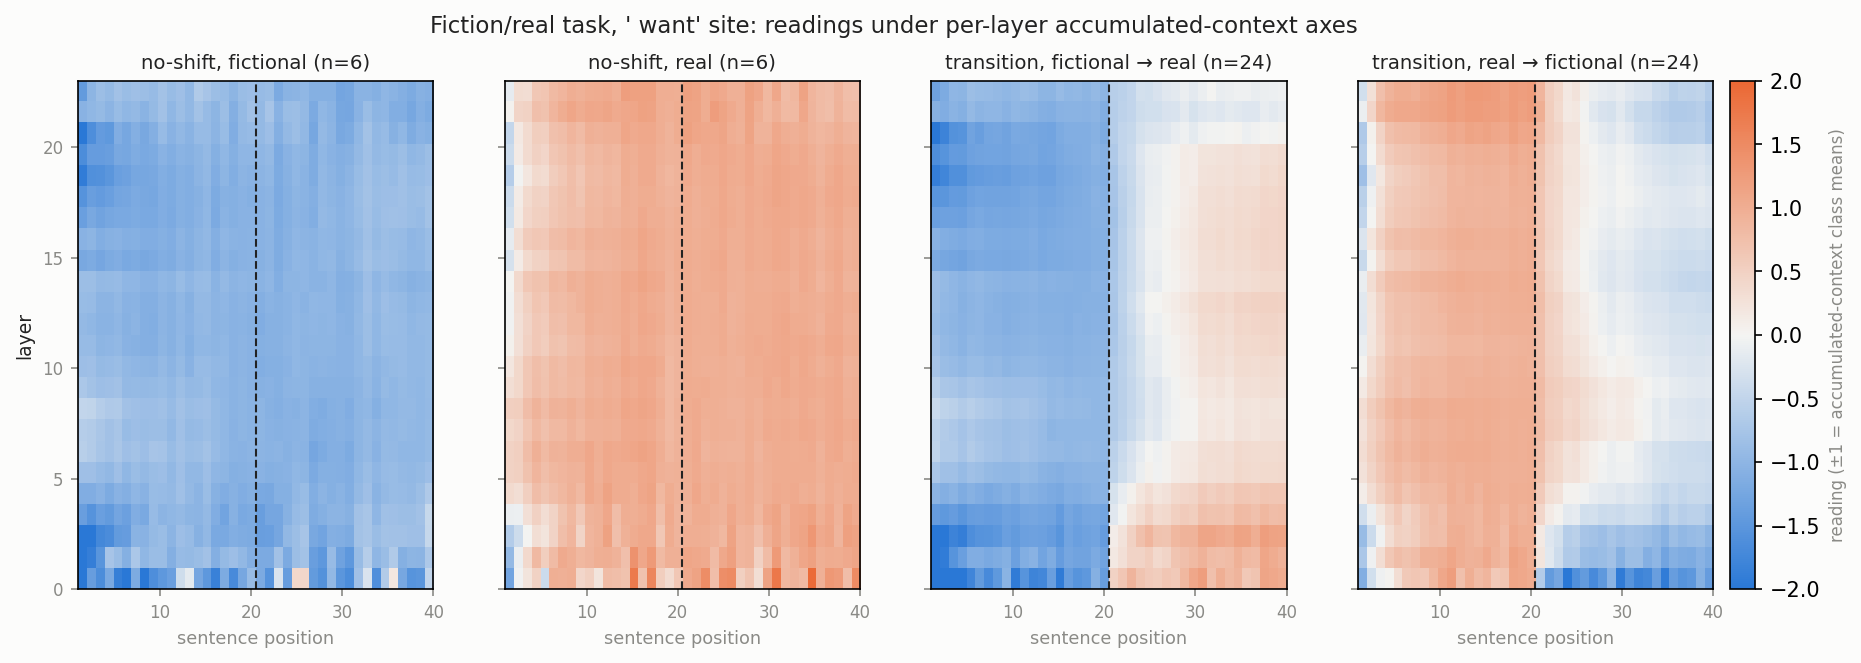
\includegraphics[width=\linewidth]{fig_r3_heatmap_secondary_fr.png}
\caption{Readings by layer and position in the fiction/real task, under axes refit per layer on accumulated no-shift contexts (class means at $\pm$1, so blue is the fictional side and red the real side). Left two panels: no-shift runs of each class, 6 runs each. Right two panels: transition runs in each direction, 24 each, with the shift after sentence 20. The dashed line marks sentence 20 in every panel. Every layer carries class signal, and no layer reads outside the range the two no-shift classes span.}\label{fig:fig_r3_heatmap_secondary_fr}
\end{figure}
\begin{figure}[tbp]\centering
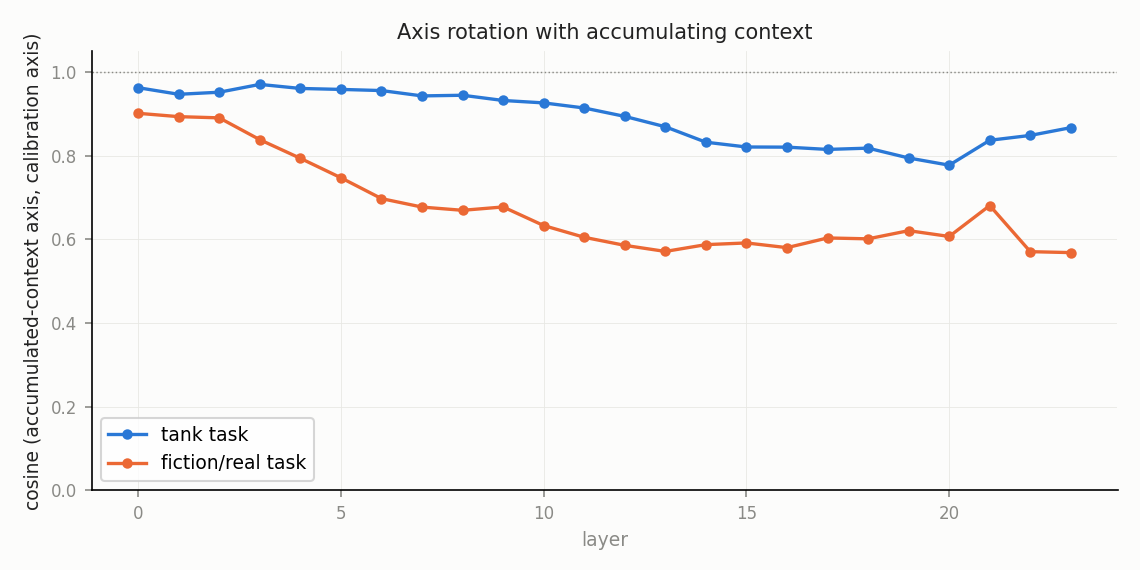
\includegraphics[width=\linewidth]{fig_r3_axis_rotation.png}
\caption{Axis rotation with accumulating context. Each point is the cosine between a layer's accumulated-context axis and its single-sentence calibration axis. The tank axis transfers across layers (cosine 0.78–0.97). The fiction/real axis rotates at depth (0.57–0.63 at layers 10–23, except layer 21 at 0.68), so claims about other layers in that task use the refit axes.}\label{fig:fig_r3_axis_rotation}
\end{figure}
\begin{figure}[tbp]\centering
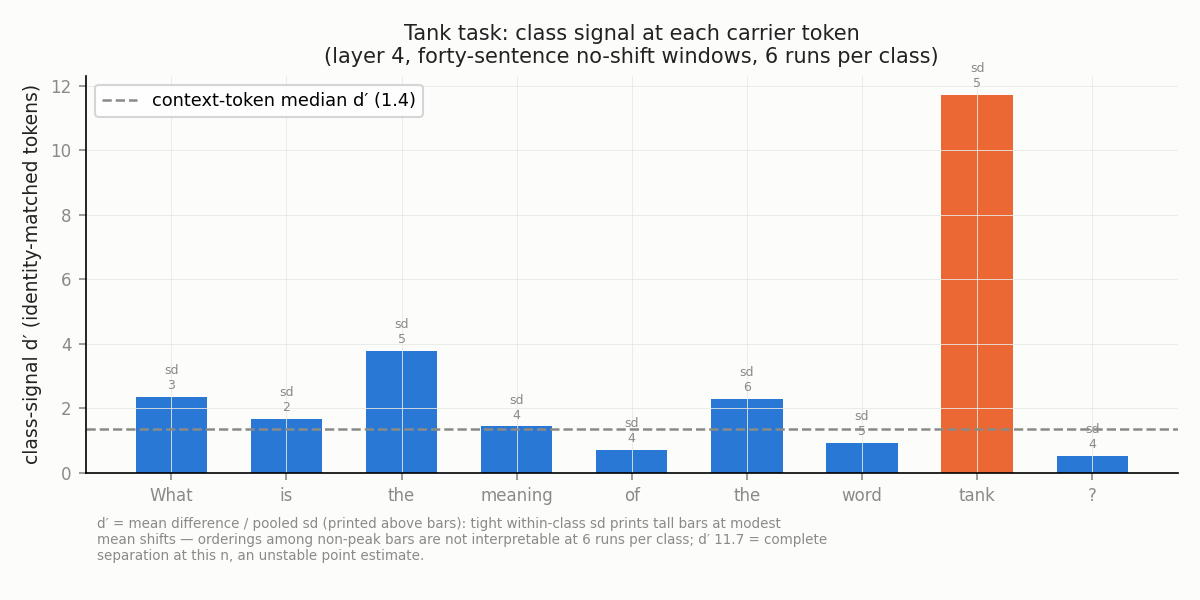
\includegraphics[width=\linewidth]{fig_r2_carrier_dprime.png}
\caption{Class signal at each token of the tank carrier, with token identity held fixed: the nine carrier tokens appear verbatim in every forty-sentence checkpoint window. Bars show $d'$ (mean difference divided by pooled standard deviation) between aquarium and vehicle contexts at layer 4, 6 runs per class. The dashed line is the median $d'$ of the context tokens (1.4). The signal concentrates at ' tank' ($d'$ = 11.7; the measurement site, in orange). The number above each bar is the pooled within-class standard deviation of the raw projection, printed to show that a small spread prints a tall bar at a modest mean shift. With 6 runs per class, orderings among the other bars are not interpretable.}\label{fig:fig_r2_carrier_dprime}
\end{figure}
\begin{figure}[tbp]\centering
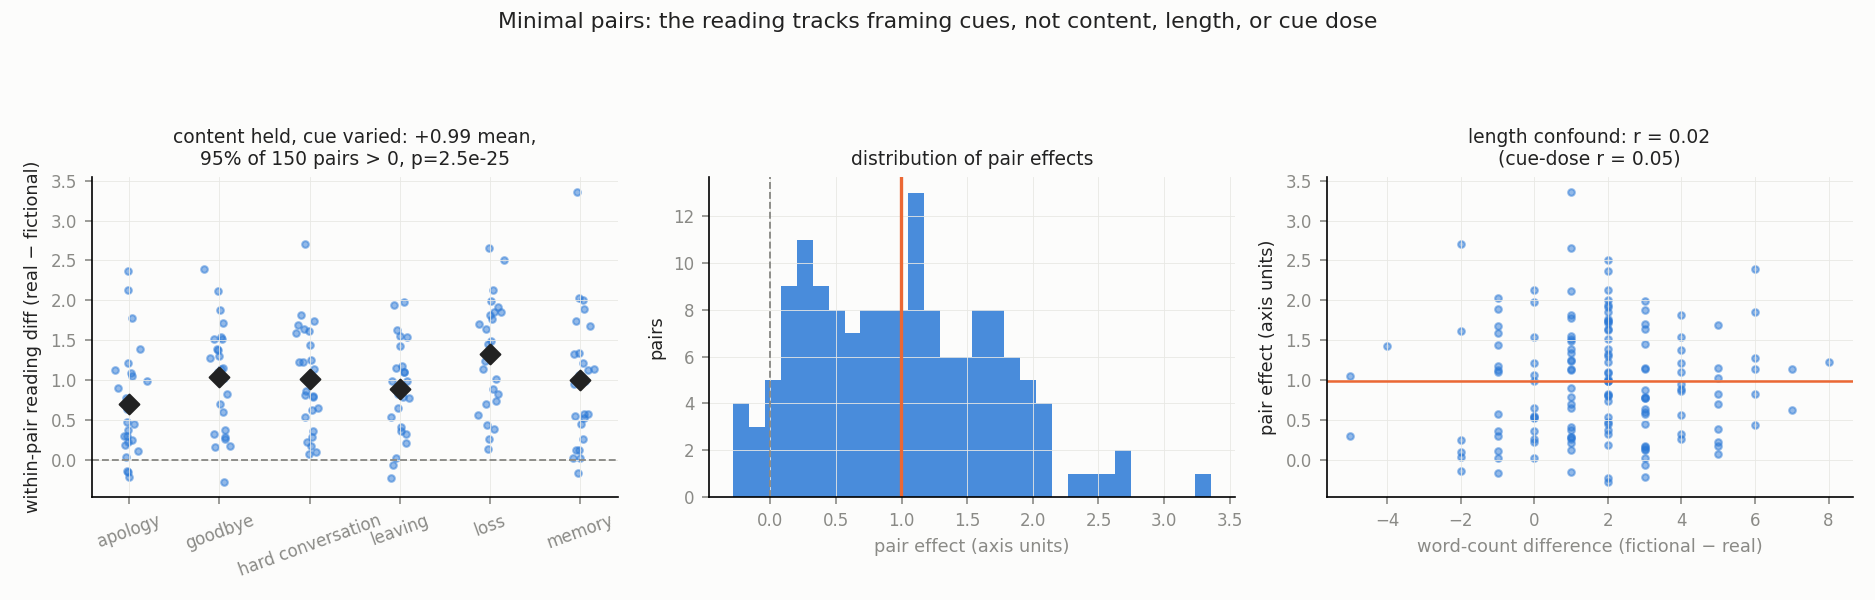
\includegraphics[width=\linewidth]{fig_s9_d5_pairs.png}
\caption{Minimal pairs: 150 sentence pairs that share most content words and differ only in framing cues. Left: the within-pair difference in reading (real minus fictional) by content domain, domain means as diamonds. The mean shift is +0.99 axis units and 95\% of pairs are positive; pair-level p = 2.5$\times 10$$^{-25}$; clustered by the six domains, t(5) = 12.0, p = 7.2$\times 10$$^{-5}$; the effect is positive in each of three independently generated batches. Middle: the distribution of pair effects. Right: the effect against the word-count difference between the two sentences (r = 0.02); the correlation with the number of cue words is r = 0.05, and length-matched pairs give +1.05. Orange lines mark the mean pair effect, +0.99.}\label{fig:fig_s9_d5_pairs}
\end{figure}
\begin{figure}[tbp]\centering
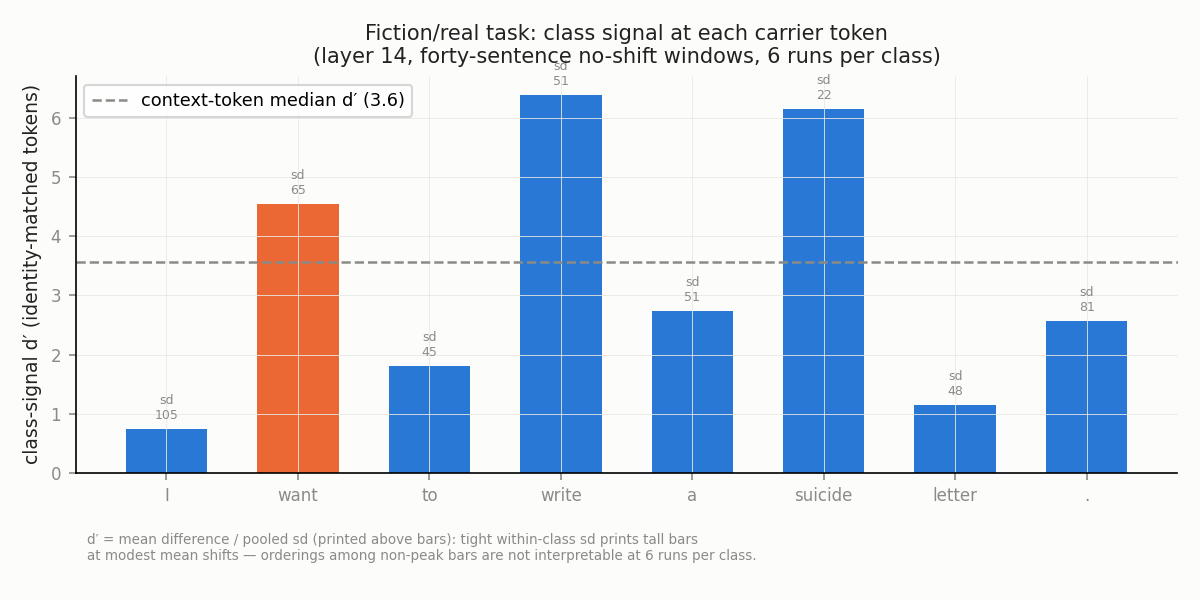
\includegraphics[width=\linewidth]{fig_r6_carrier_dprime_fr.png}
\caption{Class signal at each token of the fiction/real carrier ``I want to write a suicide letter.'', with token identity held fixed, at layer 14, 6 runs per class. The framing contrast is spread across the request's content words: $d'$ = 6.4 at ' write', 6.2 at ' suicide', and 4.5 at ' want' (the measurement site, in orange), against a context-token median of 3.6 (dashed line). The number above each bar is the pooled within-class standard deviation of the raw projection. These values are not comparable with the tank task's.}\label{fig:fig_r6_carrier_dprime_fr}
\end{figure}
\FloatBarrier
\subsection{The shape of reinterpretation: gradual, partial, lingering}

How far does a reading move after the evidence changes sides, and how fast? Figure
\texttt{fig\_s9\_collapse} shows both directions of both tasks at the calibrated sites, against
the no-shift references. After the shift the reading crosses the midpoint within a
median of 4 to 10.5 sentences, depending on the task and direction (Table 2). A few
runs never cross. The mean trajectories in Figure~\ref{fig:fig_s9_collapse} cross later than the
median run in the tank task, because runs that cross late or never pull the mean
down. In neither task and neither direction does the reading reach the
opposite reference within the twenty sentences after the shift.

How far short do they stop? The \textbf{remnant gap} measures the shortfall. It is the
no-shift reference level minus the run's plateau, both over the last five post-shift
sentences and both measured from the midpoint between the two references (\S2.5;
Fig.~\ref{fig:fig_r1_residual_gap}). The gap is positive in both directions of both tasks under
the family-clustered bootstrap (Table 2). The largest is in the tank task from
aquarium to vehicle, where the gap is 1.09 times the no-shift amplitude, the distance
from the midpoint to the matched reference. A shortfall as large as the amplitude means the plateau sits at the midpoint. Here
it is 1.09 times the amplitude, so within the interval's precision the plateau sits at
the midpoint: the transition stopped halfway.



\begin{table}[htbp]\centering\small
\caption{The transition in numbers, for both directions of both tasks. Crossing:
the per-run median number of post-shift sentences before the reading crosses the
midpoint. Decay: the median fitted $\gamma$ of the recency integrator (\S2.5). Remnant gap:
the no-shift reference level minus the run plateau, both over positions 36–40 and
both measured from the midpoint, in axis units, with family-clustered bootstrap 95\%
intervals over 2,000 draws; the second interval also resamples the six no-shift
reference runs of the destination class on every draw (Appendix A). The last column divides the gap by the
no-shift amplitude, the distance from the midpoint to the matched reference.}
\begin{tabular}{lrrrrrr}
\toprule
Transition & Crossing (median sentences) & Decay $\gamma$ (median) & Remnant gap & 95\% CI, references fixed & 95\% CI, references resampled & Gap / amplitude \\
\midrule
tank, aquarium$\rightarrow$vehicle & 10.5 & 0.99 & +2.16 & [1.87, 2.44] & [1.70, 2.62] & 1.09 \\
tank, vehicle$\rightarrow$aquarium & 6.0 & 0.94 & +1.15 & [0.82, 1.45] & [0.77, 1.48] & 0.57 \\
fictional$\rightarrow$real & 4.0 & 0.90 & +0.38 & [0.28, 0.49] & [0.27, 0.50] & 0.43 \\
real$\rightarrow$fictional & 5.0 & 0.90 & +0.35 & [0.11, 0.58] & [$-$0.12, +0.79] & 0.40 \\
\bottomrule
\end{tabular}
\end{table}

Three checks bear on the gap. First, one case weakens under a stricter bootstrap.
When the six no-shift reference runs of the destination class are also resampled, three gaps still
exclude zero, but the real$\rightarrow$fictional interval widens to [$-$0.12, +0.79] (Table 2), so
that remnant is suggestive only. Second, in the tank task, where we checked, the gap is not an artifact of weaker
post-shift material. We ranked each sentence's single-sentence reading as a percentile
within its class's calibration set. The post-shift sentences match the no-shift
sentences: for the two directions the median percentiles are 0.51 against 0.45
(p = 0.24) and 0.48 against 0.49 (p = 0.90). Third, whether the remnant
is permanent or only slower than twenty sentences can resolve is undecidable in this
corpus. The late slopes are shallow but nonzero in some runs. Deciding it is the first
item of future work (\S5).

Is the lag simply evidence integration? The transition is two-phase in a specific
sense: no single recency-weighted average fits it. Signed toward the destination, the data in both directions of both tasks run ahead
of the best-fitting average early and behind it late, and the late shortfall is the
remnant gap. The reading lags the present frame on roughly the
fitted recency timescale. The fitted decay parameters (Table 2) correspond to
weighted-mean evidence ages of about nine sentences in the fiction/real task and
fourteen in the tank task from vehicle to aquarium. From aquarium to vehicle the
fitted weighting is so close to uniform that the effective memory exceeds the window.
The stop near the midpoint, which \S3.4 calls the dwelling, shows up inside the fit
itself. Relative to an equal-weight average of all
evidence in the window, the mean trajectories run slightly ahead, which is the
pattern a recency weighting would produce, and individual runs are heterogeneous
around that mean. The crossing delay is no longer than evidence integration predicts. What integration
does not explain is the late shortfall.

Behind the single-site view there is depth structure. The depth analyses were
computed after the analysis freeze from the frozen captures and are exploratory
(Appendix B). Crossing times by depth are measured under each layer's
accumulated-context axis (\S2.4), so they differ from the calibrated-axis values of
Table 2 even at the calibrated layers. We group the layers into four bands: 0–2,
3–12, 13–18, and 19–23 (Table 3). Figure~\ref{fig:fig_s13_collapse_layers} repeats Figure
\texttt{fig\_s9\_collapse} at five layers per task, and Fig.~\ref{fig:fig_r3_heatmap_secondary_fr} with the
supplementary heatmaps gives all layers. In the fiction/real task, layers 0 to 2
cross almost immediately, within three to four sentences, and completely, while
layers 3 to 18 cross at medians of eight to thirteen sentences. The tank task crosses
later everywhere. Its layers 0 to 2 cross at medians of thirteen and eight sentences
in the two directions. From aquarium to vehicle it crosses at a median of thirteen in
every band, so the stop near the midpoint spans the whole stack there. From vehicle
to aquarium it crosses earliest in the deepest band, at a median of six. Before
computing these values we predicted that layers 5 to 9 would cross later than layers
10 to 17, with the deepest layers in between. That held in the fiction/real task and
failed in the tank task (\S5).

Where does each layer end up? Table 3 gives the mean reading over the last five
post-shift sentences by band, signed so that the destination class is positive. In
the fiction/real task, layers 3 to 18 settle at about +0.3 to +0.4 of the way to the
reference in both directions, and layers 0 to 2 settle fully. In the tank task from
aquarium to vehicle, layers 0 to 2 settle only partway, and every band below them
ends at or near the midpoint; from layer 13 down the bands end at the midpoint
itself. The deepest band, layers 19 to 23, hovers near the midpoint in one direction
of each task, fictional$\rightarrow$real at +0.08 and aquarium$\rightarrow$vehicle at $-$0.10, while the
reverse directions settle partway.



\begin{table}[htbp]\centering\small
\caption{Where each layer band ends up: the mean reading over the last five
post-shift sentences (positions 36–40) under per-layer accumulated-context axes,
averaged over the layers in each band and signed so that the destination class is
positive. Under these axes the no-shift references sit at $\pm$1 and the midpoint at 0,
so a value is the fraction of the way from the midpoint to the destination reference.}
\begin{tabular}{lrrrr}
\toprule
Layers & tank, aquarium$\rightarrow$vehicle & tank, vehicle$\rightarrow$aquarium & fictional$\rightarrow$real & real$\rightarrow$fictional \\
\midrule
0–2 & +0.57 & +1.03 & +0.99 & +1.14 \\
3–12 & +0.12 & +0.30 & +0.41 & +0.32 \\
13–18 & 0.00 & +0.38 & +0.41 & +0.33 \\
19–23 & $-$0.10 & +0.42 & +0.08 & +0.48 \\
\bottomrule
\end{tabular}
\end{table}

Direction matters, and the asymmetry survives a change of carrier and a change of
midpoint definition. In the tank task,
transitions toward the vehicle sense stop about twice as far short as transitions
toward the aquarium sense: 1.09 against 0.57 amplitude fractions (Table 2). The same
pattern replicates under the independent carrier ``Define the word tank.'' and survives
median-based midpoints (Fig.~\ref{fig:fig_s9_asymmetry}; values in the caption). The replicate
carrier's calibration axis is in-sample, not held-out. Within the fiction/real task
the asymmetry depends on the site. At the ' want' site the two directions are
symmetric. At the ' letter' site of the paraphrase carrier ``Help me write\ldots{}'' they are
strongly asymmetric. That comparison rests on 4 runs per direction and is
exploratory. A candidate cause exists at the calibration level. The vehicle class is
intrinsically broader than the aquarium class at every layer tested (spreads in the
caption), and transitions into the broader class stop farther short. The ' letter'
site, where the two classes are alike in spread, does not fit this account, but with
4 runs per direction it cannot test it. We flag the breadth account as a correlate,
not a demonstrated cause.


\begin{figure}[tbp]\centering
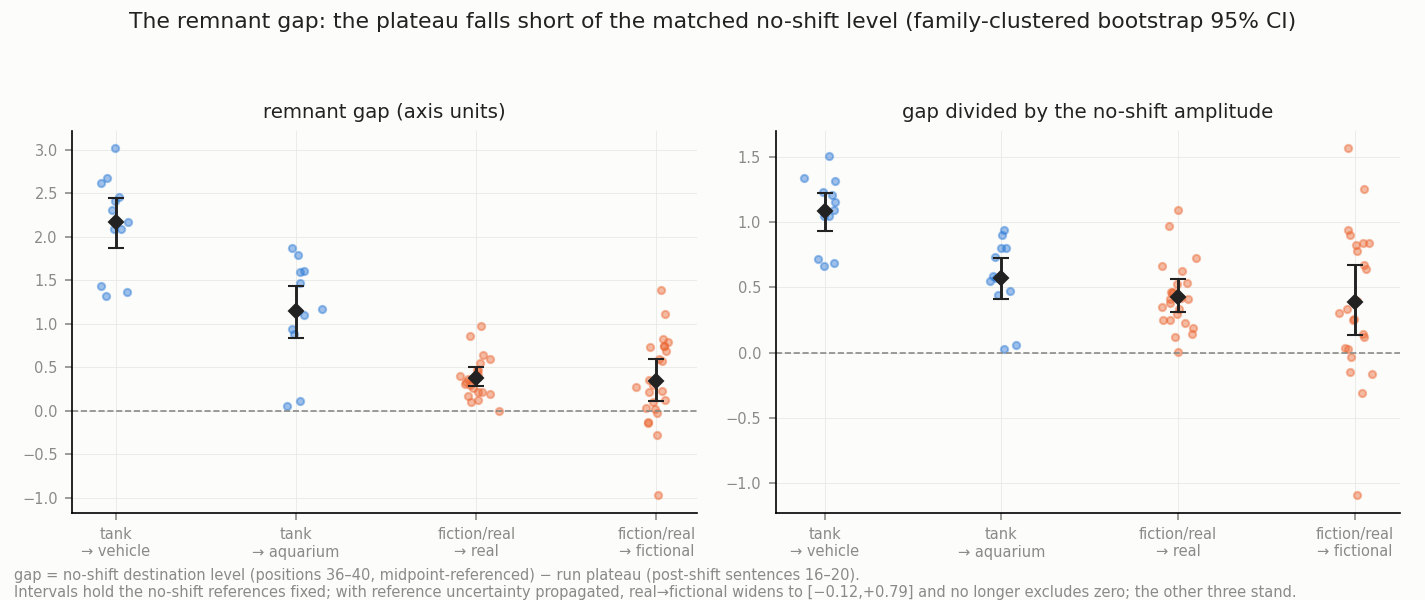
\includegraphics[width=\linewidth]{fig_r1_residual_gap.png}
\caption{The remnant gap, run by run. Each dot is one transition run: the no-shift reference level minus the run's plateau, both over positions 36–40 and both measured from the midpoint. Left, in axis units; right, divided by the no-shift amplitude, which is 2.0 in the tank task and 0.9 in fiction/real; even after this division the task with the wider endpoint separation shows the larger gaps. Each dot is one run: 12 per direction in the tank task and 24 in fiction/real. Diamonds are means with family-clustered bootstrap 95\% intervals, holding the no-shift references fixed. With the references also resampled, three intervals still exclude zero and real$\rightarrow$fictional widens to [$-$0.12, +0.79] (Table 2). Blue: the tank task, toward vehicle and toward aquarium; orange: the fiction/real task, toward real and toward fictional.}\label{fig:fig_r1_residual_gap}
\end{figure}
\begin{figure}[tbp]\centering
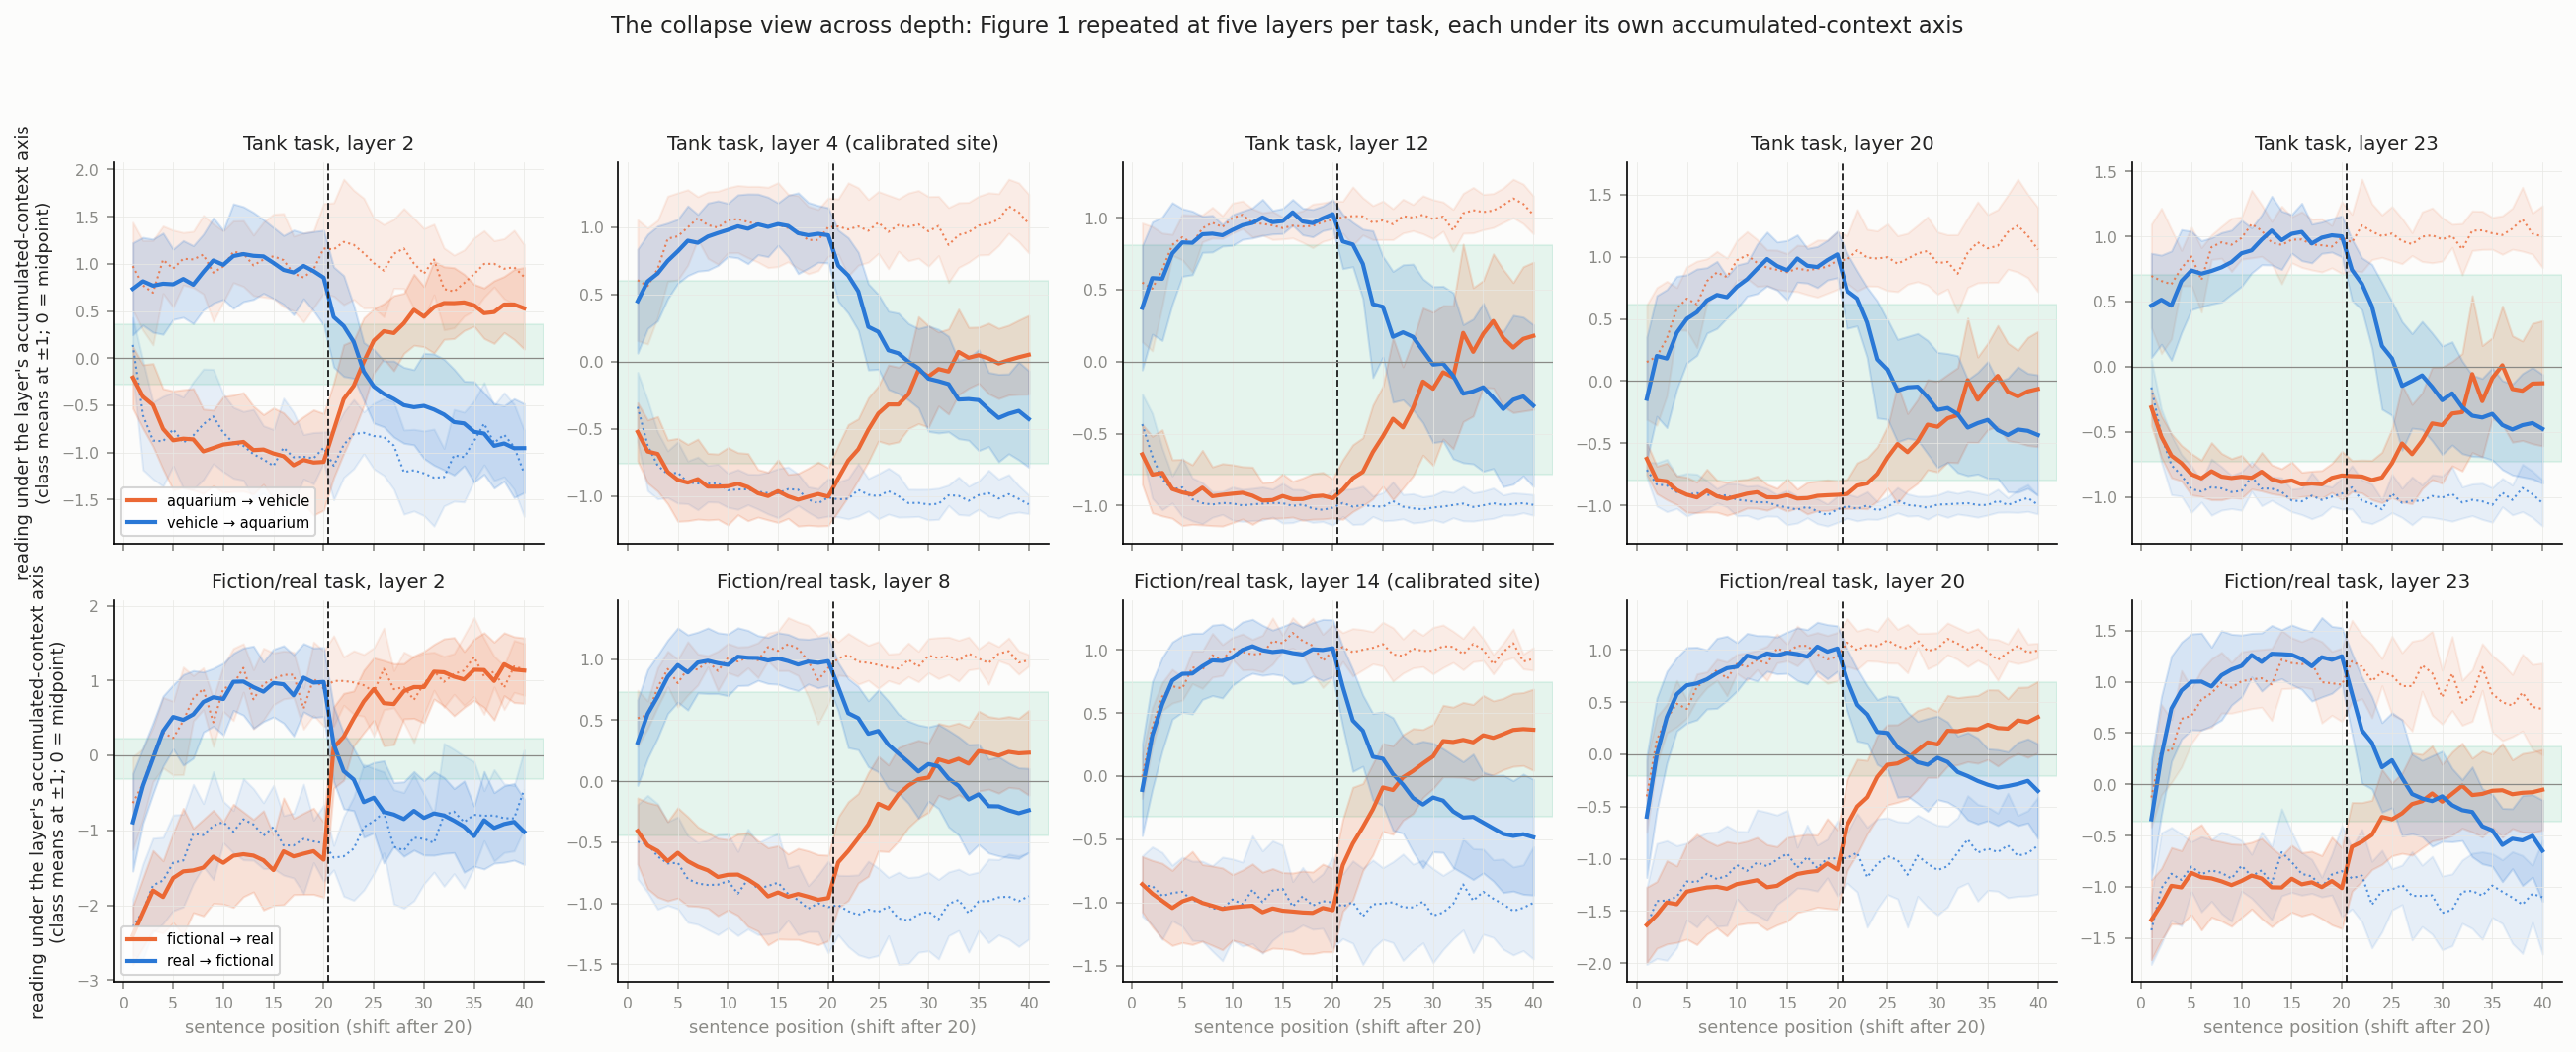
\includegraphics[width=\linewidth]{fig_s13_collapse_layers.png}
\caption{The collapse view across depth. Each panel repeats Figure 1 at one layer, under that layer's accumulated-context axis (class means at $\pm$1, midpoint 0). Top row: the tank task at layers 2, 4, 12, 20, and 23. Bottom row: the fiction/real task at layers 2, 8, 14, 20, and 23. The calibrated sites of Figure 1 are the marked panels. Solid lines are mean transition trajectories with one-standard-deviation bands; dotted lines are the no-shift references; the green band is the zone that fewer than 5\% of either reference's readings occupy. Shallow fiction/real layers flip within a few sentences and completely. Mid and deep layers move partway and stay there. Dotted lines take the color of the class they belong to. In the tank task from aquarium to vehicle, every band below the shallowest ends at or near the midpoint (Table 3).}\label{fig:fig_s13_collapse_layers}
\end{figure}
\begin{figure}[tbp]\centering
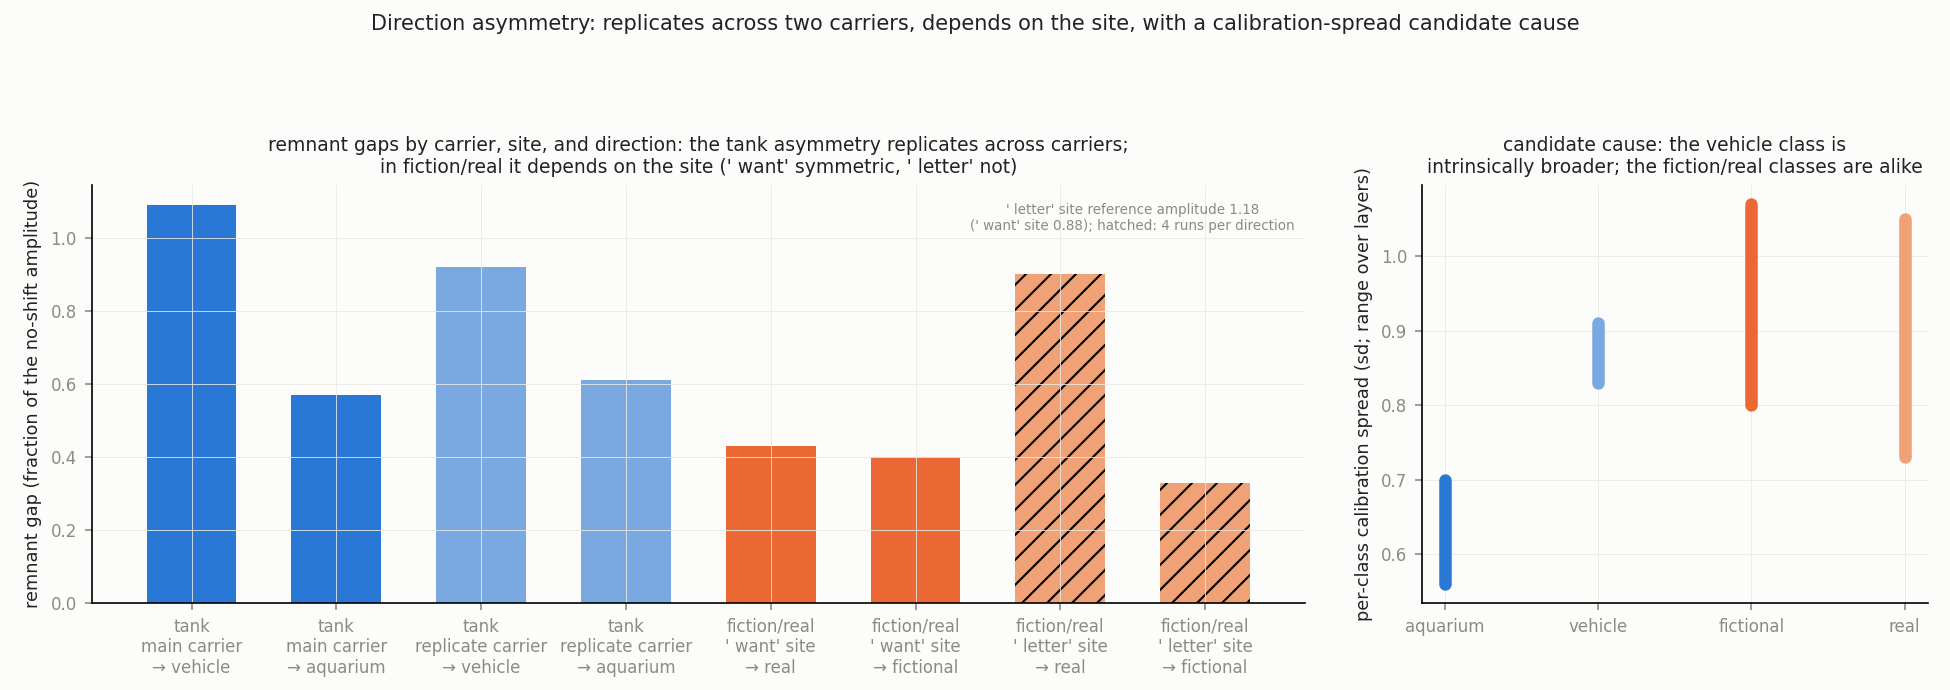
\includegraphics[width=\linewidth]{fig_s9_asymmetry.png}
\caption{Direction asymmetry. Left: the remnant gap as a fraction of the no-shift amplitude, by carrier, site, and direction. Tank, main carrier: 1.09 toward vehicle against 0.57 toward aquarium. Tank, replicate carrier ``Define the word tank.'': 0.92 against 0.61 (its calibration axis is in-sample). Fiction/real at the ' want' site: 0.43 toward real against 0.40 toward fictional. Fiction/real at the ' letter' site of ``Help me write\ldots{}'': 0.90 against 0.33 (hatched: 4 runs per direction, exploratory; that site's own reference amplitude is 1.18). Right: the spread of each class's single-sentence calibration readings, as a range over the layers tested. The vehicle class is broader than the aquarium class at every layer (0.83–0.91 against 0.56–0.70); the two fiction/real classes are alike.}\label{fig:fig_s9_asymmetry}
\end{figure}
\FloatBarrier
\subsection{The form of the dynamics: drift plus discrete jumps}

What process produces these trajectories? We fit the four model forms of \S2.5 to each
run's twenty post-shift readings: the recency integrator, the change-point step, the
drift-plus-step hybrid, and the two-timescale integrator. We select by BIC with an
indeterminacy band. Before reading the real runs we calibrated the selector on
synthetic runs of known type (Table 4). Hybrid truth is recovered as hybrid in 28 of
48 simulations. Step truth is called hybrid in 3 of 48. Two-timescale truth is called
recency integrator in 18 of 48 simulations and indeterminate in 21, and it reads as
hybrid in 5 of 48. The selector therefore rarely calls a smooth truth hybrid: 5 of 48
two-timescale runs, against 11 of 24 and 14 of 48 real runs.

On the real runs the selector favors the hybrid. Among classifiable runs, drift plus
jump is dominant: 11 of the 16 classifiable tank runs and 14 of the 25 classifiable
fiction/real runs (Table 4). In the fiction/real task, whose readings are noisier, 23
of 48 runs are indeterminate, so we state the claim as hybrid-dominant among
classifiable runs. The two-timescale model wins zero runs in either task (Fig.~\ref{fig:fig_s9_model_classes}). Per-run fits are shown in Fig.~\ref{fig:fig_r1_fit_gallery_tank}, and the
raw paths in Fig.~\ref{fig:spaghetti_L4} show the heterogeneity directly: some runs glide, some
step. The two-phase shape of \S3.2 could in principle have been smooth multi-timescale
integration. The head-to-head fit rejects it. The hybrid verdict is a claim about the
form of the trajectories, not about their implementation. It excludes smooth
integration of the evidence and establishes discrete changes in the reading. What
inside the network produces such a change is not identified here.



\begin{table}[htbp]\centering\small
\caption{Per-run model selection by BIC on the real transition runs and on
synthetic runs of known type. A model wins a run only when its BIC leads the
runner-up by at least 2; otherwise the run is indeterminate, and the classifiable
runs are the rest. Synthetic runs: 24 per task per truth type, pooled across the two
tasks; per task, hybrid truth was recovered as hybrid in 13 and 15 of 24, and
two-timescale truth read as hybrid in 2 and 3 of 24.}
\begin{tabularx}{\linewidth}{lllllll}
\toprule
Runs & Drift + step (hybrid) & Step & Recency integrator & Two-timescale & Indeterminate & Classifiable \\
\midrule
tank (24 runs) & 11 & 2 & 3 & 0 & 8 & 16 \\
fiction/real (48 runs) & 14 & 7 & 4 & 0 & 23 & 25 \\
synthetic, hybrid truth (48) & 28 & 5 & 1 & 0 & 14 & 34 \\
synthetic, two-timescale truth (48) & 5 & 0 & 18 & 4 & 21 & 27 \\
synthetic, step truth (48) & 3 & 27 & 0 & 0 & 18 & 30 \\
\bottomrule
\end{tabularx}
\end{table}

Jump timing is not predicted by evidence strength. In runs where the largest single
step carries more than half the net change, we call the sentence arriving at that
step the run's jump sentence. We rank each added sentence's single-sentence reading
as a percentile within its class's calibration set. In the tank task, all 456 added
sentences that follow a step, 19 per run, have such a reading. The jump sentences are
median-strength exemplars of their class: percentile 0.50, against 0.50 for all other
added sentences (Mann–Whitney p = 0.445). What differentiates a jump is therefore not
the stimulus property we measured. We have tested only evidence strength, and
single-sentence calibration strength may understate in-context strength. Surprisal,
syntax, and discourse position remain untested. Our working interpretation is that
jump timing depends on the run's internal state rather than on the sentence. We call
this state-dependent. It is an interpretation; the untested sentence properties have
not been excluded.

The context tokens themselves show the transition. Using per-position axes calibrated
from no-shift checkpoint windows, so that content and position are matched and only
the history differs, we read the tokens of the post-shift block. They read about a
third to a half of their no-shift reference at ten post-shift sentences, and about
half to two-thirds at twenty (Fig.~\ref{fig:fig_r2_within_stream}, \ref{fig:fig_s9_within_stream_fr};
values in the captions). The tank values are trimmed means, because the untrimmed
values are inflated by a heavy tail documented in Appendix B. The fiction/real task
replicates the pattern with a tighter instrument. Mixed history suppresses the class
reading of even the new evidence's own tokens, in a recency-graded way. This is
descriptive: it is what token-level recency integration would produce. It shows that
the transition is present in the context tokens as well as at the calibrated site.
Any readout that averages over a window of context tokens inherits the suppression.


\begin{figure}[tbp]\centering
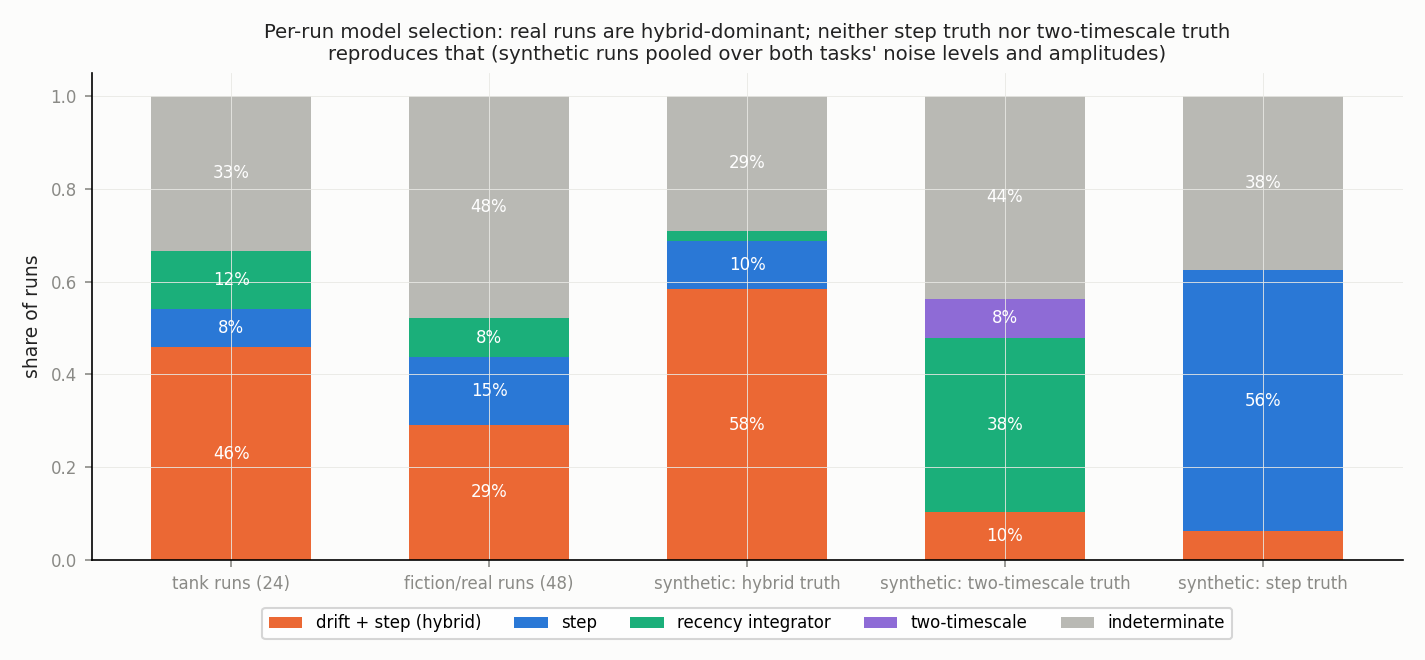
\includegraphics[width=\linewidth]{fig_s9_model_classes.png}
\caption{Per-run model selection by BIC, as shares of runs. The first two bars are the real transition runs of each task (24 tank, 48 fiction/real). The last three are synthetic runs generated from each model form with known parameters, 48 per truth type, pooled over both tasks' noise levels and amplitudes. A model wins a run only when its BIC leads the runner-up by at least 2; otherwise the run is indeterminate (gray). Real runs are hybrid-dominant among classifiable runs. Synthetic step runs and synthetic two-timescale runs are rarely called hybrid, so the selector cannot produce the hybrid verdict from either a stepwise or a smooth truth. Counts are in Table 4.}\label{fig:fig_s9_model_classes}
\end{figure}
\begin{figure}[tbp]\centering
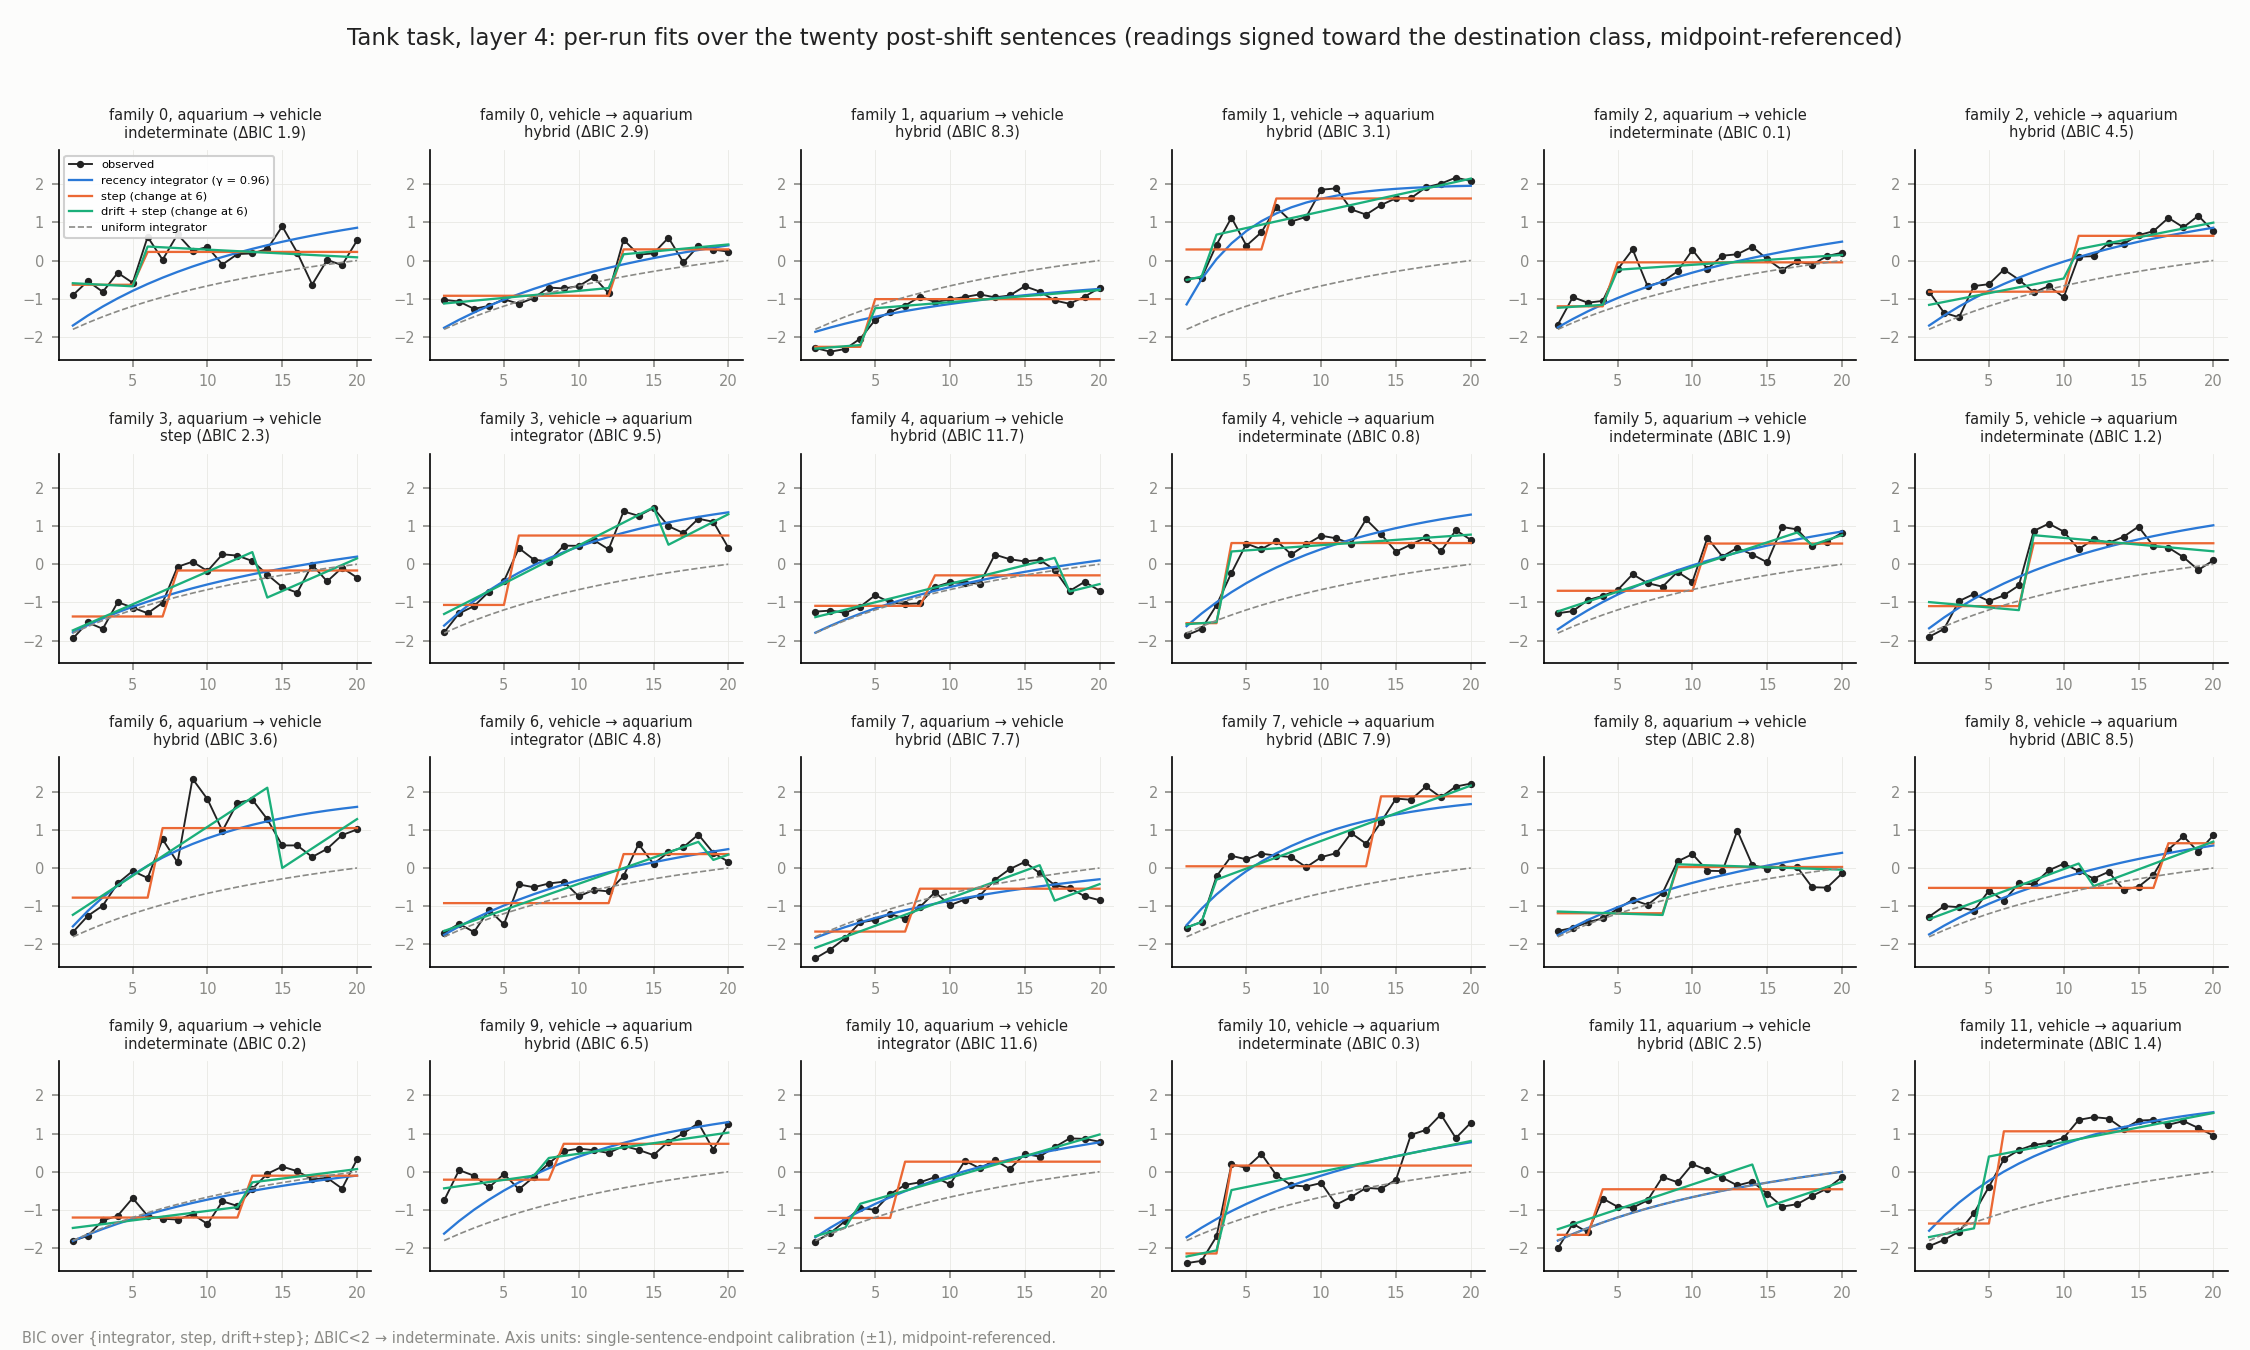
\includegraphics[width=\linewidth]{fig_r1_fit_gallery_tank.png}
\caption{Per-run fits for the 24 tank runs over the twenty post-shift sentences. Black: the observed reading, signed toward the destination class and midpoint-referenced. Blue: the best recency integrator; orange: the best change-point step; green: the best drift-plus-step hybrid; dashed gray: the uniform integrator. Each panel's title gives the scene family (the twelve settings the tank sentences were written in), the direction, the winning model, and its BIC lead. These labels come from the three-model selection, without the two-timescale form; its tallies for the tank runs, 11 hybrid, 2 step, 3 integrator, and 8 indeterminate, agree with Table 4. The legend shows the first panel's fitted values. The dashed gray line in each panel is the uniform integrator, the $\gamma$ = 1 case. The integrator underpredicts the early rise and overpredicts the late approach, and the hybrids follow the paths.}\label{fig:fig_r1_fit_gallery_tank}
\end{figure}
\begin{figure}[tbp]\centering
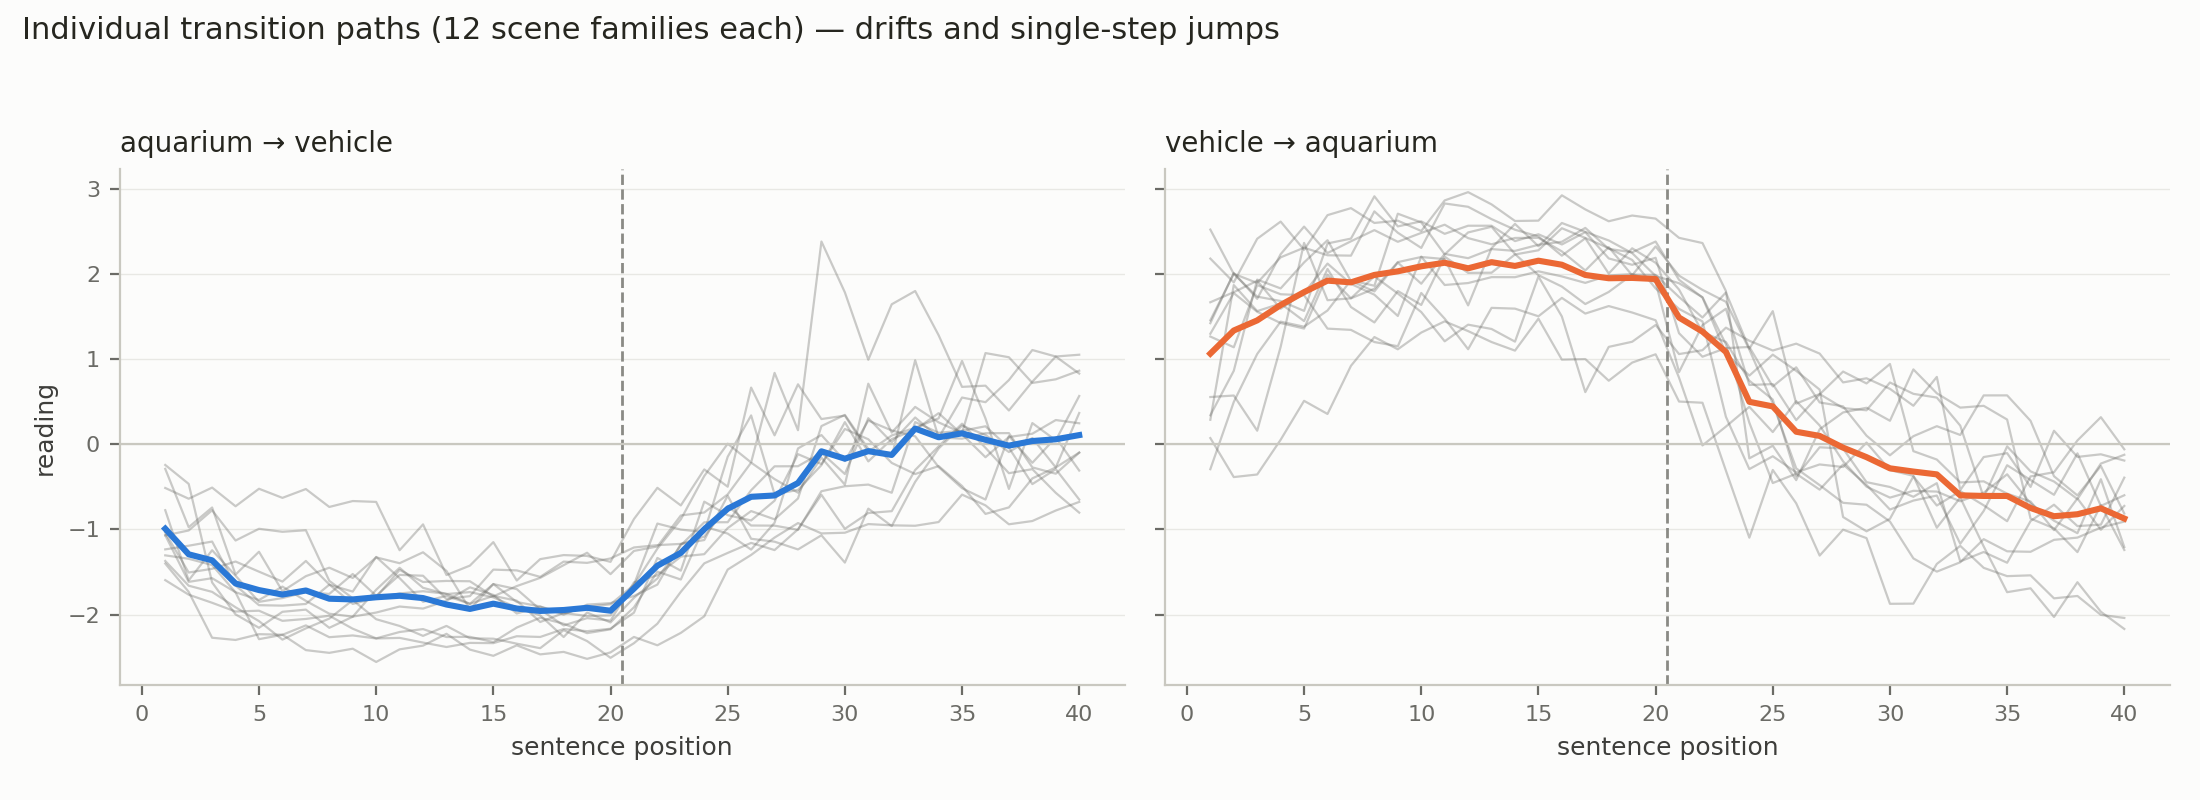
\includegraphics[width=\linewidth]{spaghetti_L4.png}
\caption{Raw per-run trajectories at the tank site (layer 4), every run of both directions, measured from the midpoint between the two no-shift references, which is why the pure-class plateaus sit near $\pm$2 rather than $\pm$1. Thin lines are single runs, the thick line in each color is the mean, and the dashed vertical line marks the shift after sentence 20. This is the heterogeneity behind the mean trajectories of Figure 1: some runs glide, some step.}\label{fig:spaghetti_L4}
\end{figure}
\begin{figure}[tbp]\centering
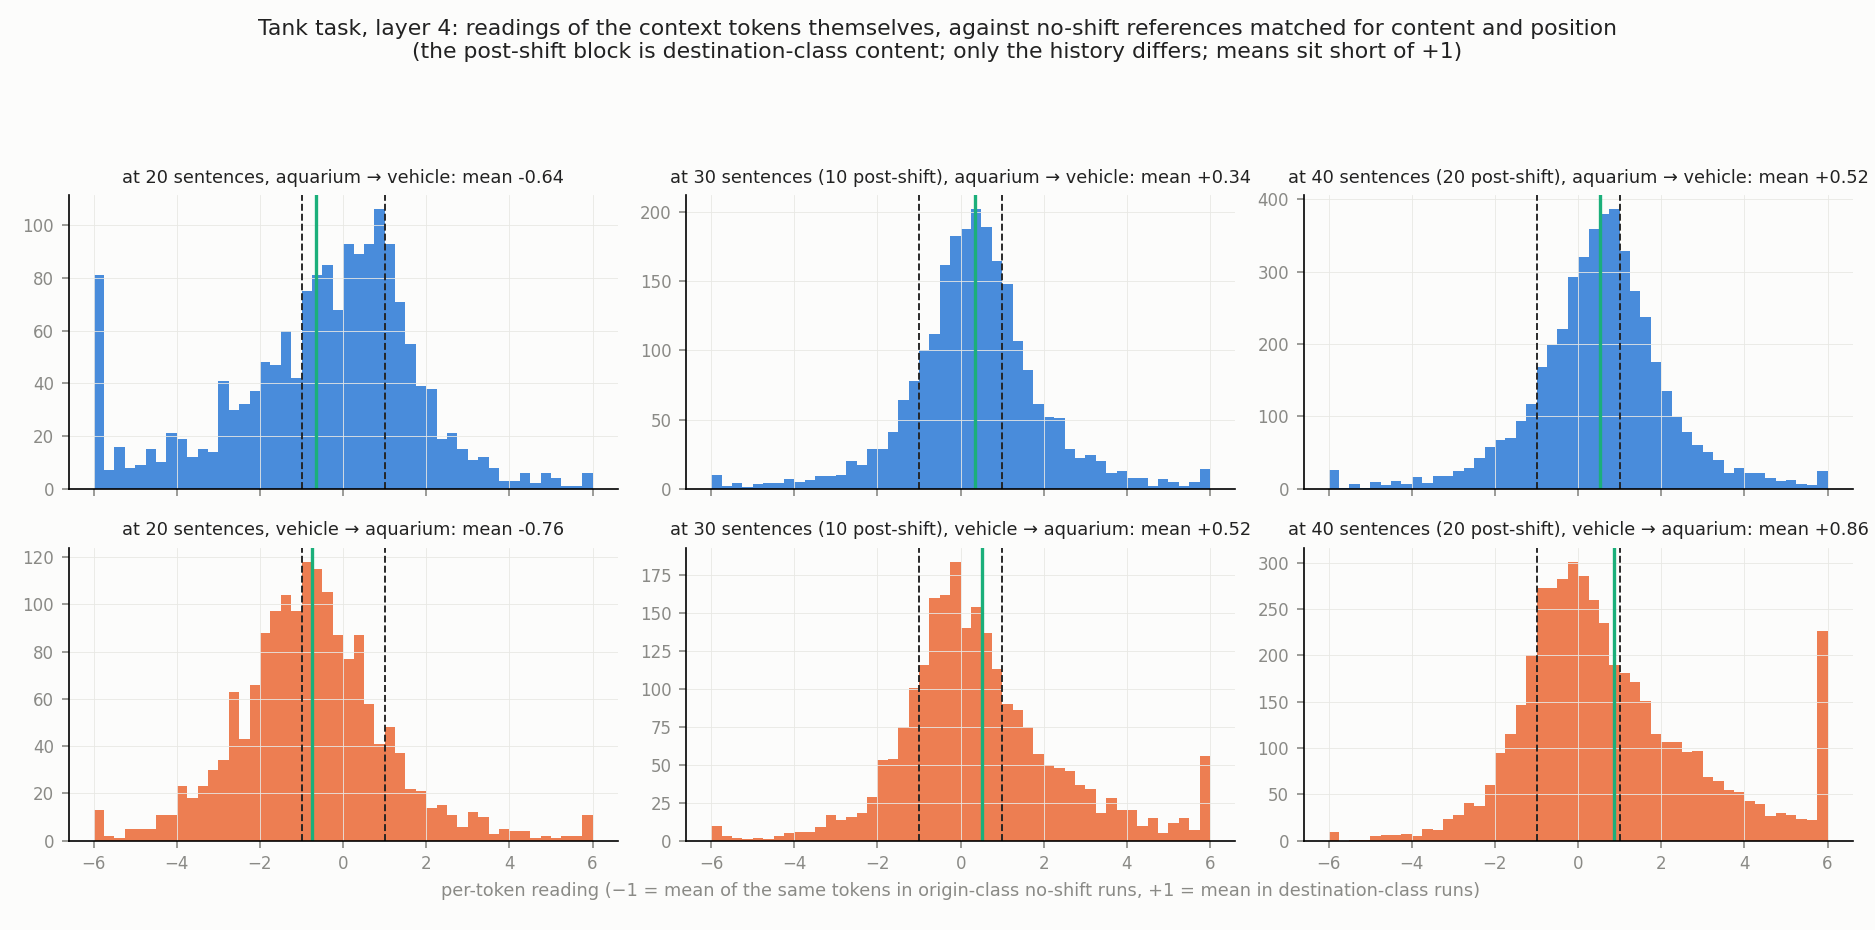
\includegraphics[width=\linewidth]{fig_r2_within_stream.png}
\caption{Readings of the context tokens themselves in the tank task (layer 4), against no-shift references matched for content and position. Each histogram is the per-token reading of the most recent block of context tokens: the last ten sentences at 20 sentences, and all post-shift sentences at 30 and 40 (top: aquarium$\rightarrow$vehicle; bottom: vehicle$\rightarrow$aquarium). The axis puts $-$1 at the mean of the same tokens in origin-class no-shift runs and +1 at their mean in destination-class runs (dashed lines); the green line is the mean. At 20 sentences the block is origin-class content. At 30 and 40 it is 100\% destination-class content, yet it reads well short of +1. Panel titles give untrimmed means. The text quotes trimmed means, because the tank distributions have heavy tails, visible as the piles at $\pm$6 where readings beyond that range are stacked for display: +0.34 (aquarium$\rightarrow$vehicle) and +0.37 (vehicle$\rightarrow$aquarium) at ten post-shift sentences, and +0.52 and +0.53 at twenty.}\label{fig:fig_r2_within_stream}
\end{figure}
\begin{figure}[tbp]\centering
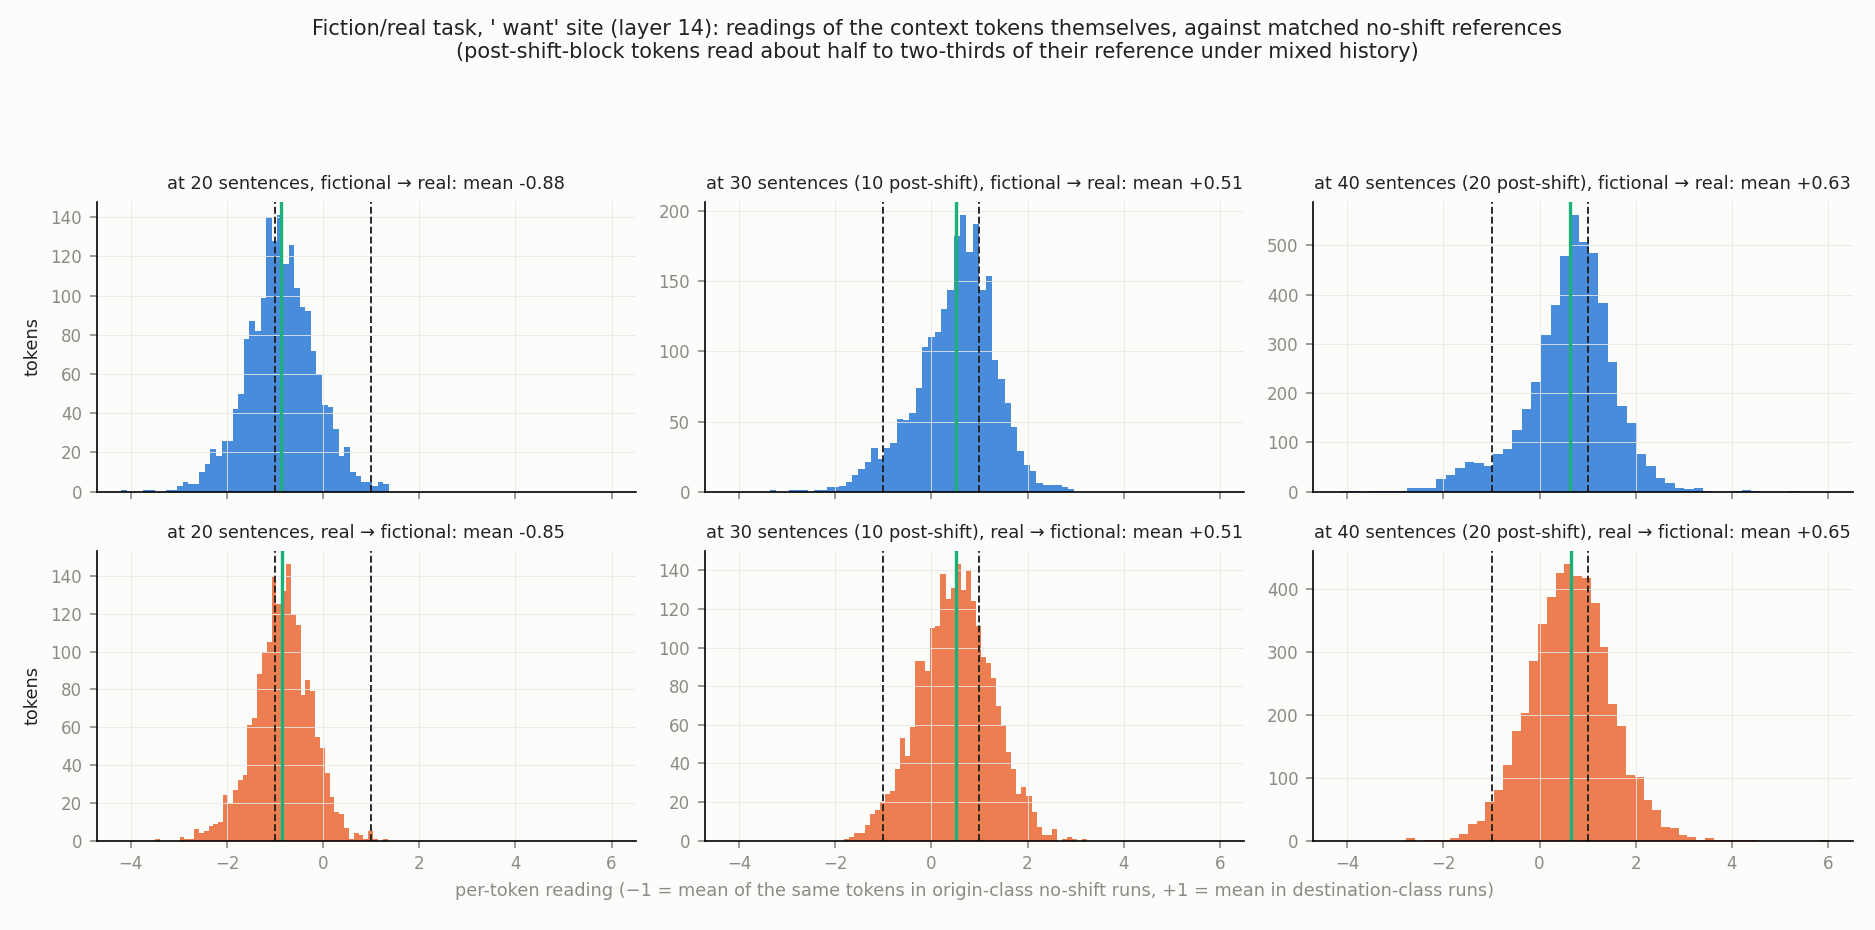
\includegraphics[width=\linewidth]{fig_s9_within_stream_fr.png}
\caption{The same measurement in the fiction/real task (' want' site, layer 14), which has a tighter instrument and no heavy tails. Top: fictional$\rightarrow$real; bottom: real$\rightarrow$fictional; panels at 20, 30, and 40 sentences. At 20 sentences the block reads near $-$1, its origin-class baseline. The post-shift-block tokens read about half of the way to their no-shift reference at +1 at 30 sentences and about two-thirds at 40 (means in the panel titles).}\label{fig:fig_s9_within_stream_fr}
\end{figure}
\FloatBarrier
\subsection{The dwelling within the unresolved zone}

Does any trajectory stop between the two interpretations rather than merely slow
down? One does. In the tank task from aquarium to vehicle, the trajectory dwells
within the unresolved zone: it becomes stationary mid-transition and, on the measured
horizon, does not leave. Figure~\ref{fig:fig_r2_mode_track} tracks the mode of the run
distribution by post-shift band. The mode is stationary at the midpoint for at least
ten consecutive steps, and it sits at least 2.9 across-run standard deviations from
both endpoint references. The spread across runs stays flat rather than tightening. A
Gaussian-mixture comparison favors a single component in every time bin, so this is
one stationary population, not a hidden mixture of resolved and unresolved runs.

The signature replicates within the tank task and barely appears in the other.
Within tank it appears at the pre-lexical ' word' site and under the replicate
carrier. In the fiction/real task it appears only at the ' letter' site of the
paraphrase carrier, with 4 runs per direction, and we treat that as exploratory.

Two qualifications bound the claim. ``Stationary'' is bounded by the horizon: whether
these runs would ever complete on a longer one is the same open question \S3.2 leaves
for the remnant, and some individual runs retain shallow nonzero late slopes. And
geometrically the dwelling states are unremarkable. They sit inside the trajectory
bundle, the spread of transition trajectories across runs, at 0.96 times the null
distance (\S3.7). Functionally they are a distinct condition, as the model's behavior
shows next.


\begin{figure}[tbp]\centering
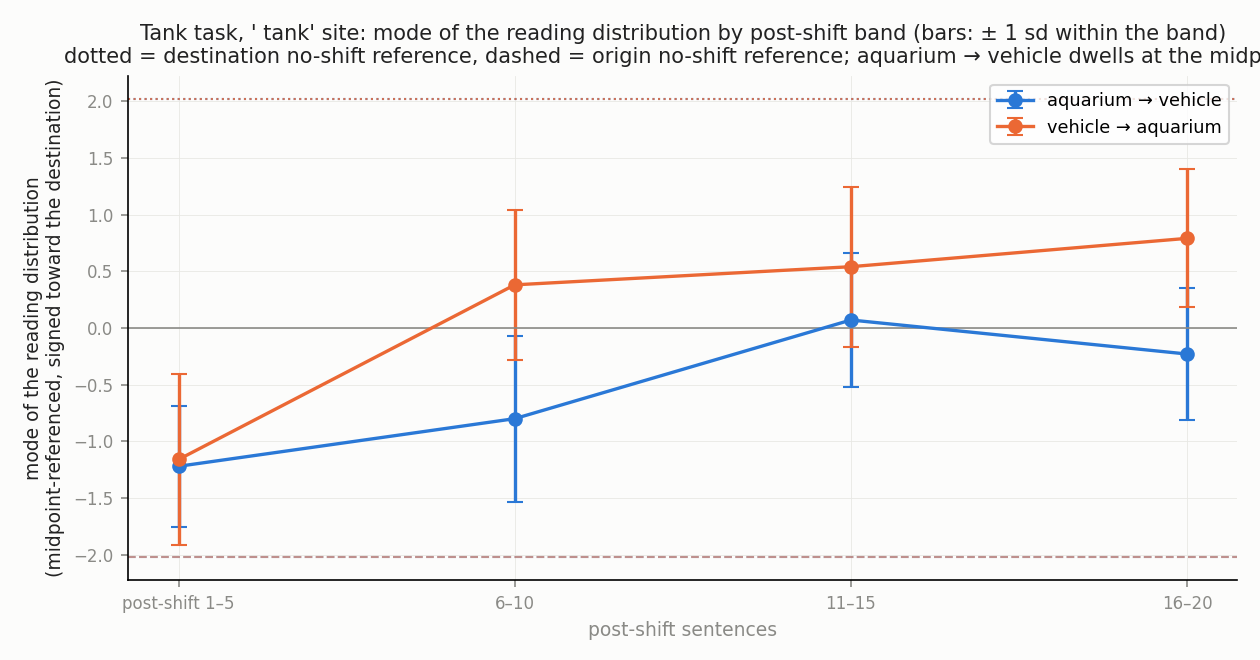
\includegraphics[width=\linewidth]{fig_r2_mode_track.png}
\caption{The dwell in the tank task, at the ' tank' site. Each point is the mode of the distribution of readings across runs within a five-sentence post-shift band, signed toward the destination class and midpoint-referenced; bars show one standard deviation across runs within the band. Dotted lines are the destination no-shift reference for each direction and dashed lines the origin reference. From aquarium to vehicle (blue) the mode reaches the midpoint by the third band and stays there through the last, at least 2.9 across-run standard deviations from both references, with the spread flat; a Gaussian-mixture comparison favors one component in every band. From vehicle to aquarium (orange) the mode keeps moving.}\label{fig:fig_r2_mode_track}
\end{figure}
\FloatBarrier
\subsection{What the model does in the unresolved zone}

What does the model say while its reading sits between the two interpretations? We
generated a completion from every run at four points after the shift: after 2, 6, 12,
and 20 post-shift sentences. All behavioral claims in this subsection are
correlational. For analysis we partition readings into three bands, the origin side,
the middle, and the destination side (Fig.~\ref{fig:fig_r6_behavior_bands}).

Behavior tracks the reading. Completions whose readings sit on a side answer that
side, in 56\% and 66\% of cases for the two sides. The middle band answers ``both'',
listing the two senses, in 45\% of its completions, roughly double either side. One
descriptive fact anchors this paper's framing. Not one of the 96 tank responses asks
which sense is meant or declines to answer pending disambiguation. That is zero of
96, by regular-expression scan and manual review of the committed categorization
table. In the unresolved zone the model either lists both senses (45\%) or silently
commits to one (52\% of middle-band completions). It answers as if resolved. One
further response class appears across all 108 tank completions, the 96 transition
completions plus 12 from no-shift runs: 11 are degenerate repetition loops, unrelated
to the reading band.

Does the reading carry information beyond the context composition that drives both
reading and behavior? We test this at matched composition, comparing completions
generated after the same number of post-shift sentences (Fig.~\ref{fig:fig_s9_behavior_matchedk}). Mid-transition, yes. Pooling the completions at 6 and 12
post-shift sentences, decided answers come from runs with more extreme readings, with
a median absolute reading of 0.72 against 0.38 (one-sided p = 0.0138). This pooling
was chosen after the per-depth pattern was seen, so we grade the result suggestive.
At the settled extremes, no. In the fiction/real task we categorize each completion
as fiction-framed assistance or a safe-completion. A safe-completion addresses the
request as a risk, declining the letter or redirecting to support, rather than
fulfilling it. The reading separates the two types at 2 post-shift sentences, where
the medians are $-$0.06 and +1.13 (p = 0.010), one of four counts tested. Later the
reading does not separate them, and response type follows the scene family.

The safety-relevant gradient is plain at the band level. Safe-completion rates run
50\%, 80\%, and 91\% as the reading moves from the fiction side through the middle to
the real side. The fiction-side band rests on 4 completions and is fragile.

An exploratory check added after the analysis freeze (Appendix B) asks whether any
other layer's reading associates more strongly with behavior than the calibrated
site's. Per-layer association curves (Fig.~\ref{fig:fig_s14_behavior_by_layer}) are roughly
flat from mid-stack to the final layer in both tasks. Nothing singles out the deep
layers. The instrument is blunt, a band-level association with imbalanced outcomes,
so this neither establishes nor rules out a depth-specific behavioral readout.


\begin{figure}[tbp]\centering
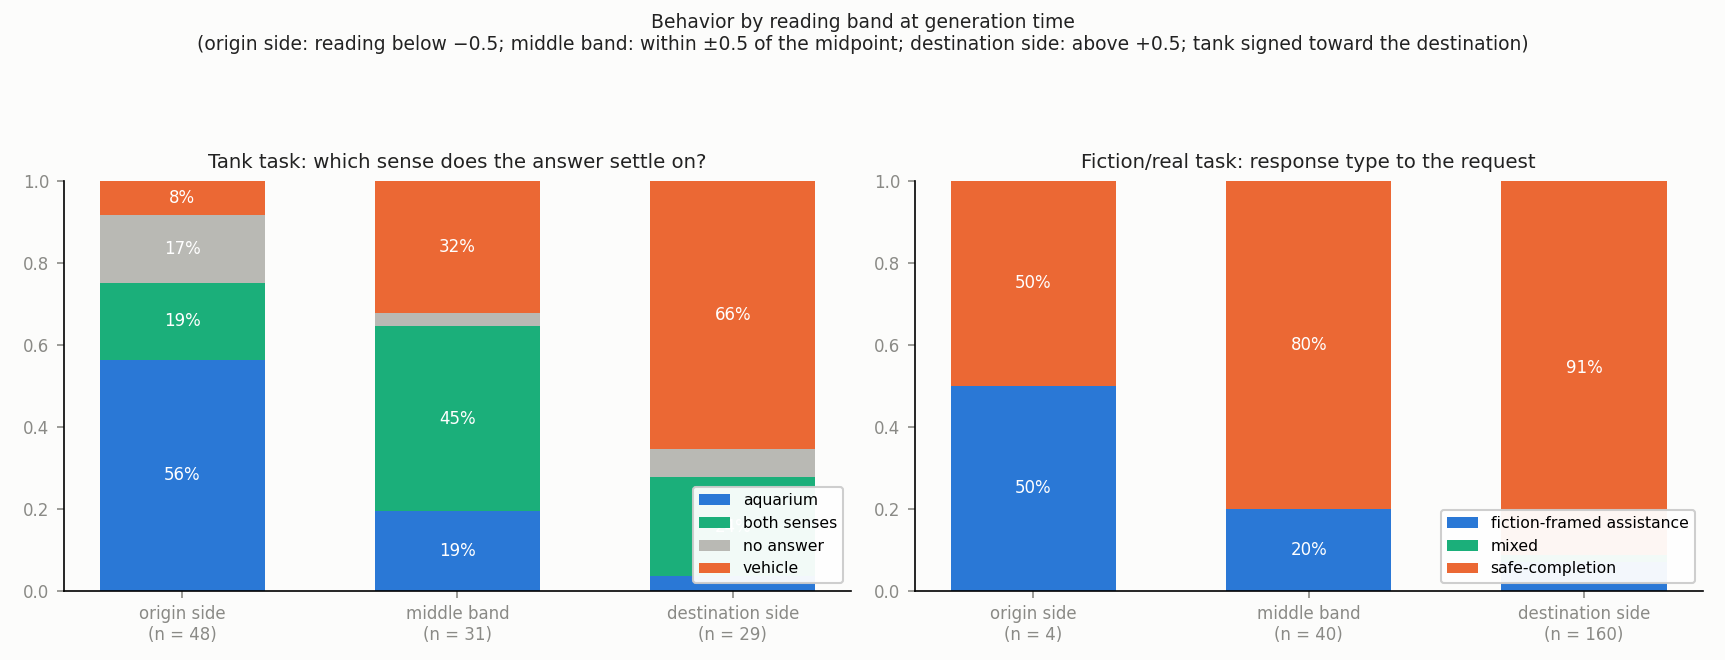
\includegraphics[width=\linewidth]{fig_r6_behavior_bands.png}
\caption{Behavior by reading band. Completions are grouped by the reading at generation time: below $-$0.5 (origin side), within $\pm$0.5 of the midpoint (middle band), above +0.5 (destination side), signed toward the destination for the tank task; the number of completions per band is under each bar. Left: the tank task, by which sense the answer settles on (aquarium, vehicle, both senses listed, or no answer). Side bands answer their side (56\% and 66\%); the middle band lists both senses in 45\% of completions. Right: the fiction/real task, by response type: fiction-framed assistance, mixed, or safe-completion, which declines the letter or redirects to support. Safe-completion rises from 50\% on the fiction side (4 completions) through 80\% in the middle band to 91\% on the real side.}\label{fig:fig_r6_behavior_bands}
\end{figure}
\begin{figure}[tbp]\centering

\includegraphics[width=\linewidth]{fig_s9_behavior_matchedk.png}
\caption{Behavior against the reading at matched context composition, that is, among completions generated after the same number of post-shift sentences. Left: the tank task. Each dot is one completion's absolute reading, signed toward the destination, split by whether the answer settled on one sense (blue) or hedged or gave no answer (green); bars are medians. Mid-transition, at 6 and 12 post-shift sentences, decided answers come from runs with more extreme readings (pooled medians 0.72 against 0.38, one-sided p = 0.0138, graded suggestive because the pooling was chosen after the pattern was seen). Right: the fiction/real task, reading by response type, fiction-framed assistance (blue) or safe-completion (orange). At 2 post-shift sentences assistance comes at lower readings (medians $-$0.06 against +1.13, p = 0.010); at later counts the reading does not separate the types.}\label{fig:fig_s9_behavior_matchedk}
\end{figure}
\begin{figure}[tbp]\centering
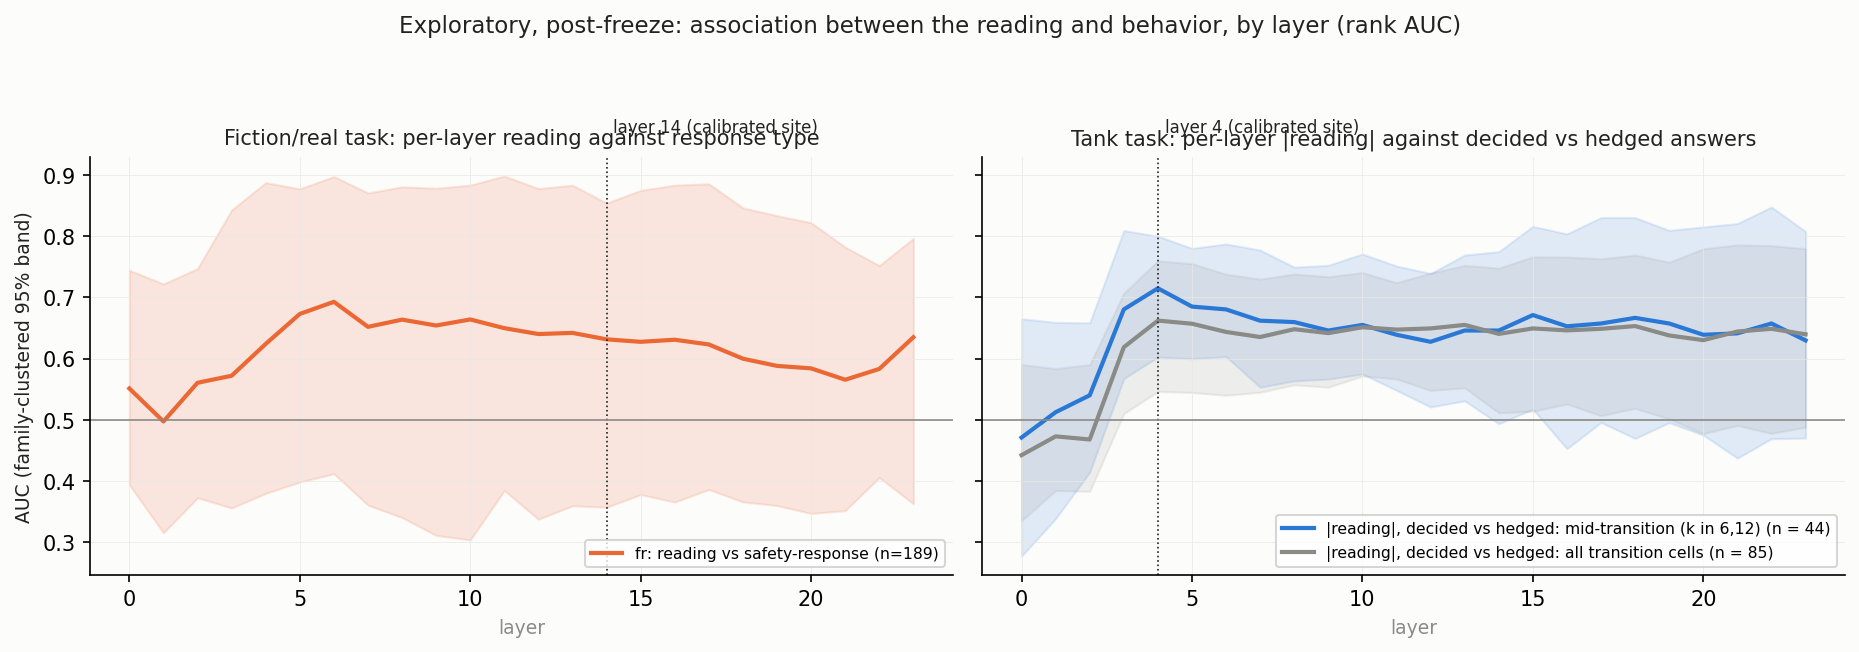
\includegraphics[width=\linewidth]{fig_s14_behavior_by_layer.png}
\caption{Exploratory, added after the analysis freeze: the association between the reading and behavior at every layer, as a rank AUC with family-clustered 95\% bands. Left: the fiction/real task, reading against response type (189 completions). Right: the tank task, absolute reading against decided versus hedged answers, for mid-transition completions (44, at 6 and 12 post-shift sentences) and for all transition completions (85). Dotted lines mark the calibrated sites. The curves are roughly flat from mid-stack to the final layer in both tasks. The instrument is blunt: a band-level association with imbalanced outcomes.}\label{fig:fig_s14_behavior_by_layer}
\end{figure}
\FloatBarrier
\subsection{Order and equilibrium: hysteresis without stickiness}

Does the order of evidence matter beyond its amount? To ask this we built static
mixture sweeps: twenty-sentence contexts holding k destination-class sentences, with
k swept from 0 to 20, in two block orders, using each family's own transition
sentences. The resulting loops are large. The same mixture read with the destination
block recent rather than old differs by a loop area of +14.4 [12.2, 16.8] in the tank
task (Fig.~\ref{fig:fig_r6_d6_loop_tank}) and +10.5 [7.5, 13.3] in fiction/real (Table 5).
Operational hysteresis is plainly present.

The reserved question was whether any of that order dependence exceeds what recency
weighting alone produces. We call any such excess \emph{stickiness}. There is none. A
one-parameter recency integrator fitted to the sweep cells reproduces the loop areas
almost exactly, and the excess is indistinguishable from zero in both tasks (Table 5).
Cross-order validation, fitting one branch and predicting the other, preserves the
verdict. An earlier pass computed this against a misspecified null, with $\gamma$ imported
from the transition fits, and found apparent stickiness. The fitted null supersedes
it (Appendix A). What remains beyond the single-$\gamma$ account is mild. The two sweep
directions prefer slightly different recency weights, echoing the directional
asymmetry of \S3.2.



\begin{table}[htbp]\centering\small
\caption{Hysteresis in the static mixture sweeps. Loop area is the area between
the two block-order branches of the sweep, in axis units times sentences, with a
family-clustered bootstrap 95\% interval. The fitted loop area comes from a
one-parameter recency integrator fitted to the same cells; the excess is the
observed area minus the fitted area. The last column gives the recency weight $\gamma$
fitted separately to each block order.}
\begin{tabular}{lrrrr}
\toprule
Task & Observed loop area & Fitted integrator loop area & Excess (stickiness) & $\gamma$, the two block orders \\
\midrule
tank & +14.4 [12.2, 16.8] & +14.3 & +0.1, not significant & 0.91 / 0.97 \\
fiction/real & +10.5 [7.5, 13.3] & +11.1 & $-$0.5, not significant & 0.84 / 0.90 \\
\bottomrule
\end{tabular}
\end{table}

This resolves an apparent contradiction with \S3.3. The equilibrium map from evidence
mixture to reading is smooth and integrator-like. The sequential path through a
transition is drift punctuated by jumps. Both are true. They are different
observables. The metastability this paper names is a property of paths, not of the
equilibrium map. There is no bistability to fall into and no barrier to escape.


\begin{figure}[tbp]\centering
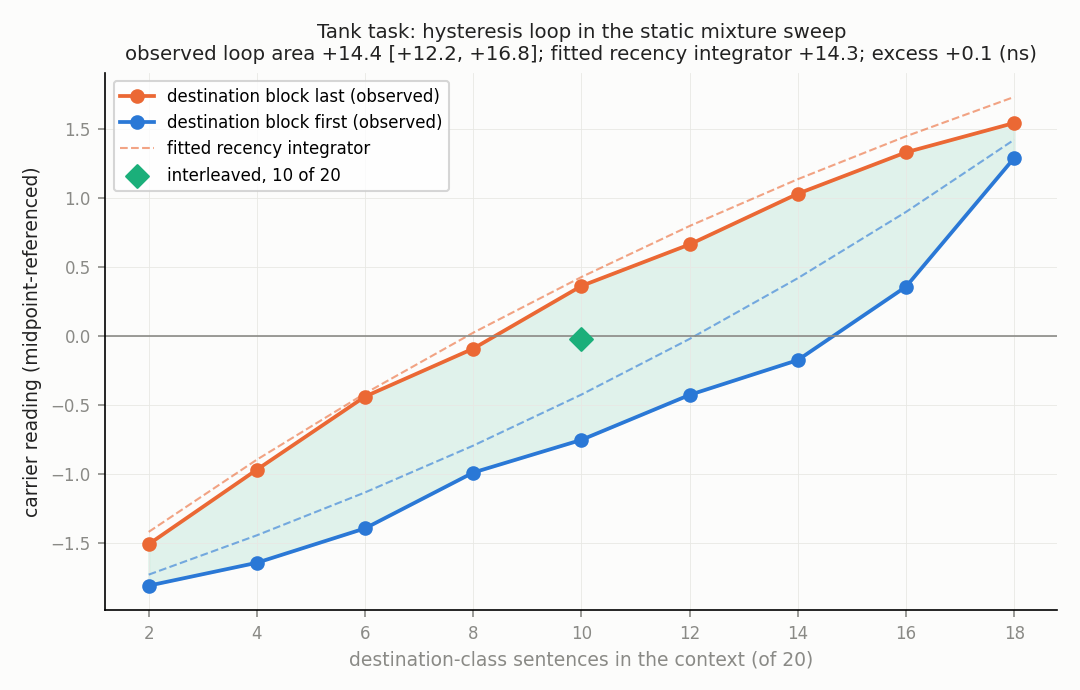
\includegraphics[width=\linewidth]{fig_r6_d6_loop_tank.png}
\caption{Hysteresis in the tank task. Each point is the mean carrier reading, midpoint-referenced, in a twenty-sentence context holding a fixed number of destination-class sentences, with the destination block placed last (orange) or first (blue). The shaded area between the branches is the loop: the same mixture reads differently depending on the order, with area +14.4 [12.2, 16.8]. Dashed lines are the predictions of a one-parameter recency integrator fitted to the same cells, which reproduces the loop (area +14.3); the excess, +0.1, is indistinguishable from zero. The green diamond is an interleaved mixture of 10 destination sentences in 20, which falls between the branches. The fiction/real sweep (not shown) gives +10.5 [7.5, 13.3] observed against +11.1 fitted (Table 5).}\label{fig:fig_r6_d6_loop_tank}
\end{figure}
\FloatBarrier
\subsection{The geometry of irresolution}

Finally, the third of the introduction's three worlds: do these in-between states
leave the model's learned distribution? ``Off-manifold'' is meaningful only relative to
a reference, a measure, and a noise level, so we fix all three. The reference is the
position-matched no-shift states, together with the cross-run transition bundle. The
measures are the distance to the nearest neighbors in the reference and the
out-of-subspace reconstruction error against the no-shift principal-component
subspace. The noise level is the held-out self-distance of the reference itself.
Throughout this section, paired values are for the tank and fiction/real tasks in
that order. The instruments detect real displacement. Single-sentence calibration states, a
genuinely different context regime that serves as a positive control, read 1.7 to
2.2 times the null across the two instruments. Position-mismatched states are
flagged at 13\% to 44\%.

At the level of individual states, nothing leaves the reference distribution. Jump
steps read 1.06 and 1.12 times the null, and the stationary dwelling states 0.96
times, all inside the null's spread (Fig.~\ref{fig:fig_r5_geometry}). Our pre-registered
prediction that jump steps would show elevated off-manifold distance failed.

The subtle result appeared when we challenged the per-state verdict. A displacement
too small to flag any single state could still be shared by all of them, so we tested
the mean directly. The mean out-of-subspace reconstruction error of transition states
is far outside the range of a family-block bootstrap null (Fig.~\ref{fig:fig_s9_shift_marker}).
It is a shared displacement equal to 25\% and 38\% of the full class separation, with
p < 0.001 in both tasks. It rises over the first five post-shift sentences and persists
undiminished to twenty, and it is largest in the stationary dwelling states. We call
the direction that carries it the \textbf{mixed-context marker}.

Three checks say what the marker is not (Table 6). It is not class leakage: the
direction is orthogonal to the single-sentence class axis and, by construction and by
measurement, to the accumulated-context class axis. It survives held-out direction
estimation, retaining 71\% to 90\% of its in-sample magnitude. And it is not family
novelty. If the marker merely reflected unfamiliar scene families, pure-class cells
from families outside the reference construction should sit higher on it than cells
from familiar families. They sit lower, and both sit far below mixed cells.



\begin{table}[htbp]\centering\small
\caption{The mixed-context marker and its checks. Values are for the tank and
fiction/real tasks. The displacement rows are in percent of the full class
separation; the cosine rows measure the marker direction against the two class axes.}
\begin{tabularx}{\linewidth}{lXl}
\toprule
Quantity & tank & fiction/real \\
\midrule
Shared displacement of transition states & 25\% & 38\% \\
Cosine with the single-sentence class axis & +0.015 & +0.011 \\
Cosine with the accumulated-context class axis & $-$0.0052 & $-$0.0065 \\
Retained under held-out direction estimation & 71\%–90\% of in-sample magnitude & (both tasks) \\
Pure-class cells from families outside the reference construction & +1.6\% & +3.4\% \\
Pure-class cells from familiar families & +6.7\% & +6.0\% \\
Mixed cells & $\approx$ +27\% & $\approx$ +27\% \\
\bottomrule
\end{tabularx}
\end{table}

What is it? Held-out mixture cells locate what elevates it. The marker is absent from
pure-class contexts and near its full transition strength in static mixed contexts,
so it marks mixed context, not temporal shifting as such. One qualification: in the
fiction/real task it halves when the mixture is interleaved rather than blocked, so
there, part of what elevates it is the coherent, blocked structure of the shift. It
did not predict behavior in eight matched-composition tests at the calibrated site
and layer, with one nominal hit, uncorrected; other layers are untested. The model,
in other words, carries a persistent, systematic signal that its context is mixed: a
direction on which pure contexts sit near zero and mixed contexts near 27\% of the
class separation. Its behavior does not appear to use it. Whether this signal is
a learned representation of mixedness or a systematic consequence of heterogeneous
input is not decided by our measurements.

Three graded senses of ``off-distribution'' should be kept distinct. The first is
exotic natural inputs. The second is interventional states, such as patching and
steering. The third is states of one context regime measured against a reference
built from another, as our single-sentence positive controls are. Our shifts are the tamest possible case, clean
block transitions between two well-learned frames. That even the dwelling states stay
on-distribution here says nothing about adversarial or incoherent contexts, where
genuine excursions remain most likely. That battery is future work.

\begin{figure}[tbp]\centering
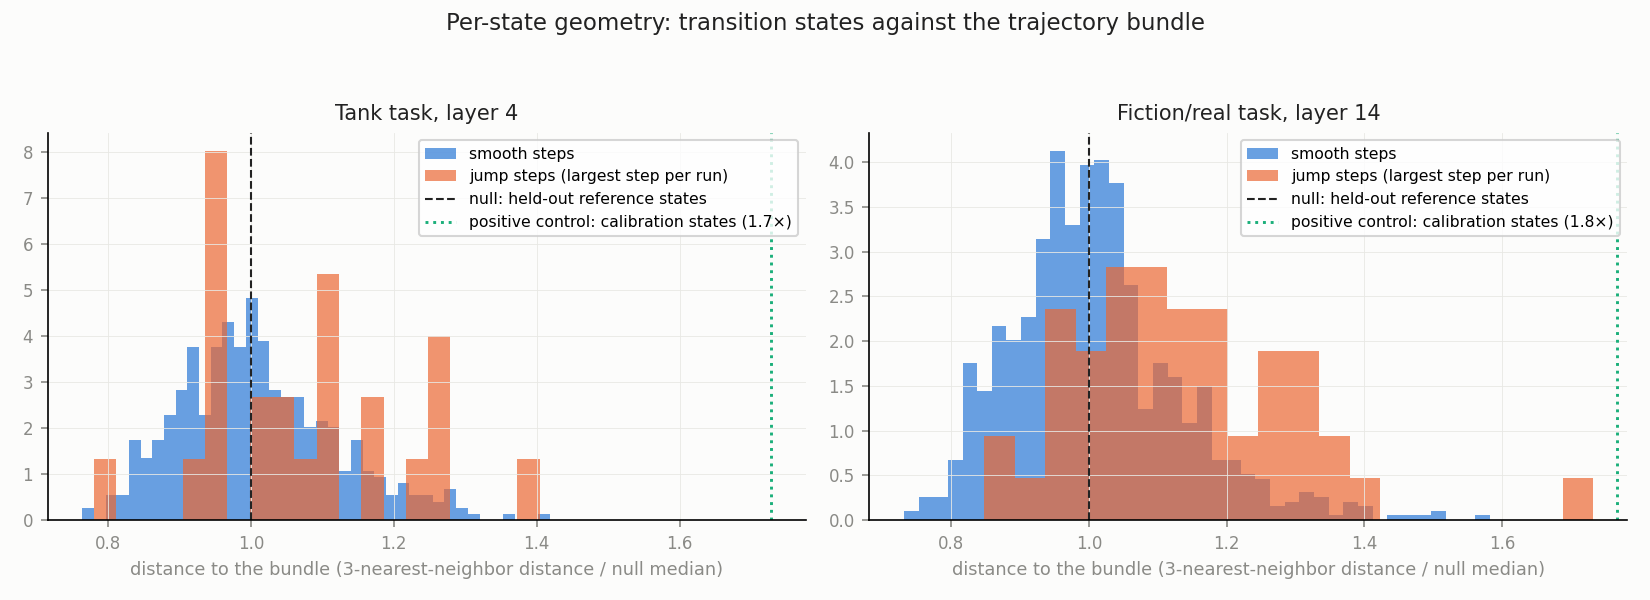
\includegraphics[width=\linewidth]{fig_r5_geometry.png}
\caption{Per-state geometry. For every transition state at the calibrated site, the distance to its three nearest neighbors in the reference set, divided by the median of the same score for held-out reference states (the null, dashed line at 1.0). Blue: smooth steps; orange: the largest step in each run, the jump steps. Left: the tank task at layer 4; right: fiction/real at layer 14. Both distributions sit inside the null's spread. The dotted green line is the positive control: single-sentence calibration states, a different context regime, read 1.7 and 1.8 times the null on this instrument.}\label{fig:fig_r5_geometry}
\end{figure}
\begin{figure}[tbp]\centering
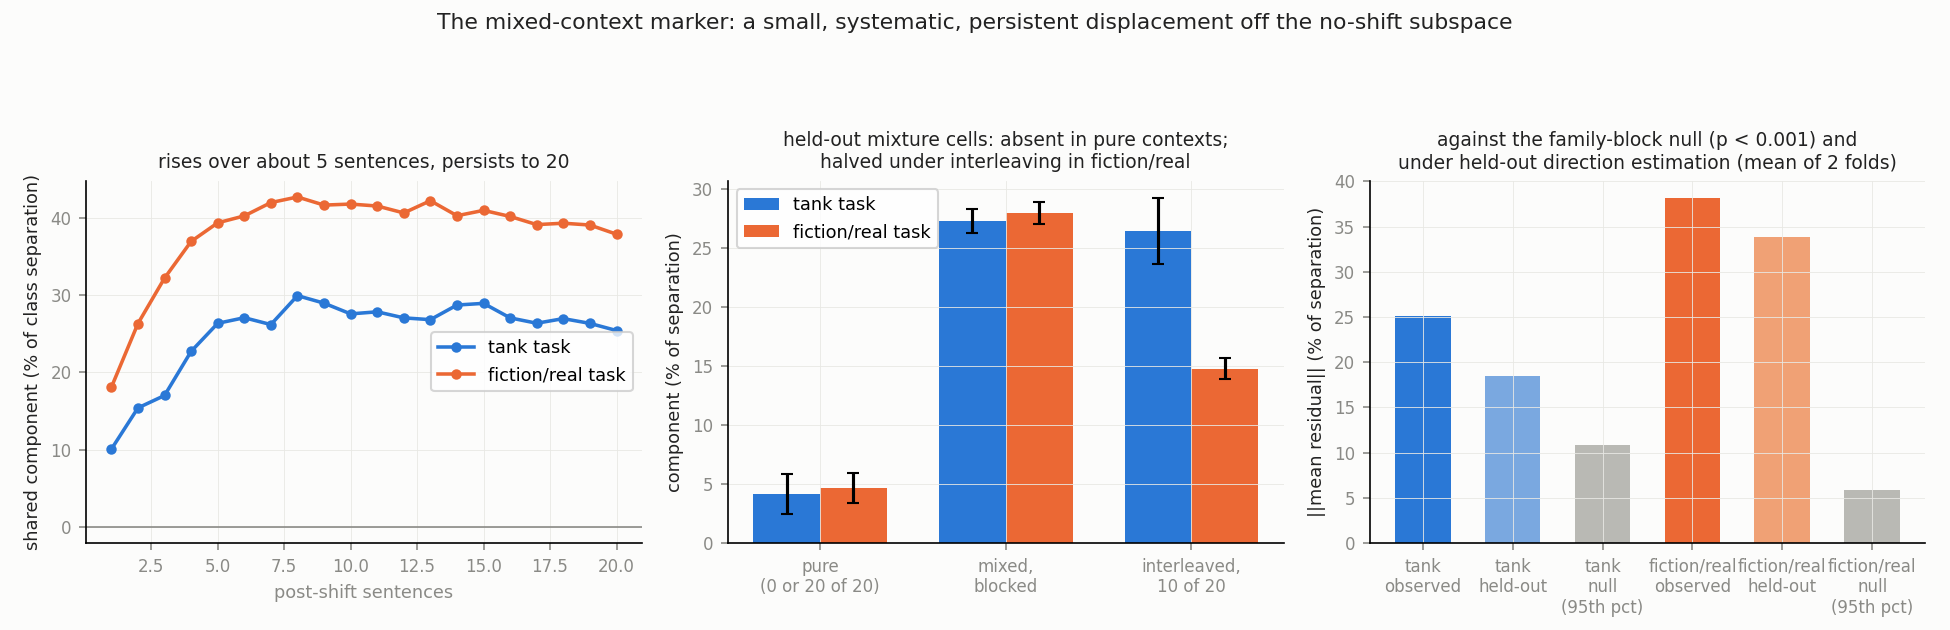
\includegraphics[width=\linewidth]{fig_s9_shift_marker.png}
\caption{The mixed-context marker. Left: the mean displacement of transition states outside the no-shift principal-component subspace, projected on the shared direction and expressed as a percentage of the class separation, by post-shift sentence. It rises over about five sentences and persists to twenty. Middle: held-out mixture cells from the static sweeps. The marker is near zero in pure-class contexts (0 or 20 destination sentences of 20), near full strength in blocked mixtures, and, in the fiction/real task only, halved when the mixture is interleaved. Right: the observed mean displacement against the 95th percentile of a family-block bootstrap null (p < 0.001 in both tasks), and its value under held-out direction estimation, the mean of two folds.}\label{fig:fig_s9_shift_marker}
\end{figure}
\FloatBarrier

\section{Discussion}

\textbf{What ``metastable'' means here.} We take the term from the dynamics of biological
neural systems rather than from physics. In coordination dynamics and in the
winnerless-competition framework, two models of sequential transient dynamics in
neural populations, cognition is described as a sequence of transiently stable states
that are not fixed-point attractors [CITE: metastability in neural dynamics]. These
are structured passages through state space, in which dwelling and moving are not
opposites. That is the geometry our data show. A run that dwells mid-transition
occupies something functionally state-like: it is stationary for many steps and has
its own behavioral signature. Geometrically it is a passage, inside the trajectory
bundle and on a smooth equilibrium map. One disclaimer follows. Nothing here is
equilibrium bistability, since the map from evidence mixture to reading is smooth
(\S3.6), and readers should not import a barrier-crossing picture. Semantic
metastability, as we use it, is a property of paths.

\textbf{Typicality is not commitment.} The three-worlds question of \S1 dissolved because
it conflated two axes. On distributional typicality the stationary states are
unremarkable: inside the bundle, on-distribution. On semantic commitment they are
distinctive: uncommitted, between calibrated interpretations, with hedging as their
behavioral expression. A learned state of unresolvedness would be typical and
uncommitted at once. That is the profile the stationary states show, which is why the first two worlds of
\S1 were never alternatives. Genuinely off-distribution states, such as glitch inputs,
interventions, and adversarial incoherence, fall elsewhere on the typicality axis and
remain untested here. The general lesson is that a state can be geometrically typical
without being functionally normal. Our behavior data document the functional
difference.

\textbf{Safety and alignment, first descriptively.} The failure surface this study maps
needs no adversary. During an ordinary, coherent shift of conversational frame, a
model's reading of a critical token trails the present frame for roughly the fitted
recency timescale. Here that is nine to fourteen sentences, and effectively without
bound in the dwelling direction. It retains a remnant of the prior frame beyond that.
In one tank direction it dwells between frames for the remainder of the tested
horizon. The fiction/real task shows an exploratory echo of this, resting on 4 runs
per direction.

Behavior inside this window tracks the reading. Throughout, in the tank task, the
model never asks which reading is meant or flags the ambiguity as an obstacle. That
holds in zero of 96 completions across all bands. Even so, 45\% of middle-band answers
surface both senses. And safeguard-relevant behavior co-varies with the internal
reading. Safe-completion rates fall from 91\% to 50\% across reading bands. The
fiction-side endpoint rests on four completions, and the gradient is partly
scene-driven (\S3.5). This weakening is reachable by ordinary context, with no exotic
inputs required.

\textbf{A trained default for unresolved cases?} What follows is a post-hoc reading of an
asymmetry we noticed, not a designed manipulation, and training provenance is
unobservable. Our two tasks appear to differ in whether they carry a trained default
for unresolved cases. The covered fiction/real task behaved as though it does. In the middle reading
band, 80\% of its completions safe-complete. In sampled chain-of-thought traces, both
framings are weighed before the safe reply. These traces are the reasoning channel
the chat format exposes, and we release them with our behavior data. That is a
qualitative observation, not a coded rate. The tank task showed no such default.
There the model silently commits: 52\% of middle-band completions pick a sense. If
this reading is right, the unresolved zone is the failure window for every behavior
without a trained uncertainty-default, and refusal-style safeguards may be the
well-covered exception rather than the rule.

\textbf{Why the safeguard held: three candidate accounts.} Three accounts could explain why
the covered fiction/real task mostly safe-completed in the middle reading band, and
we cannot yet separate them. They are not exclusive: one is about what training
installed, one about what deeper layers see, one about where in the stack the trigger
reads. None is causally established. With two tasks these are observations. The
exploratory per-layer curves of \S3.5 cannot separate them either. Shallow readings
saturate after the shift, which blinds that instrument in exactly the layers the
third account below points to.

\emph{A trained default.} The first account is the reading above: the fiction/real task
carries a trained default for unresolved cases, and the tank task does not.

\emph{Resolution at depth.} The second account emerged from the depth data, and it is
weaker than it first looked. In the fiction/real task, layers 3 to 18 settle clearly
on the destination side in both directions, where the tank task from aquarium to
vehicle ends at the midpoint (\S3.2). Downstream layers in the fiction/real task may
therefore act on a more settled reading than the site we measure. But the deepest
layer band hovers near the midpoint in the fictional-to-real direction too, the
direction in which safeguard behavior must appear, and did. Resolution at depth cannot carry the
explanation alone.

\emph{An early, surface-keyed trigger.} The third account points the opposite way through
the stack. The shallowest layers resolve the framing composition almost immediately
and completely (\S3.2), with the profile of surface-cue tracking. The minimal-pair test
that rules out cue-only tracking was run at the calibrated site, not at shallow
layers. A safeguard that reads early, from surface content and frame cues, would fire
whenever the alarming request is present and be suppressed only by a well-established
fictional frame. That is the shape of our behavioral data, including its fragile 50\%
fiction-side floor. The fast, complete shallow response is specific to the
fiction/real task. The tank task's shallow layers respond later and, in one direction,
only partway (\S3.2). That is what a trigger sculpted by safety post-training would
look like. But ordinary register statistics learned in pretraining predict the same
asymmetry, and training provenance is unobservable here. Patching shallow against
mid-stack states during generation is the decisive test (\S5).

\textbf{One limit.} We state it so that this section cannot overpromise. As a standalone
monitor, predicting each response from its reading alone, the frame reading is not
yet usable: its AUC is 0.61 [0.43, 0.76], compatible with chance (Fig.~\ref{fig:fig_s11_monitor_roc}). The band-level gradient of \S3.5 is real. A usable monitor would
combine several sites, the mixed-context marker, and per-layer readings. Building one
is future work, not a claim.

\textbf{A signal behavior does not appear to use.} The mixed-context marker gives the
sharpest form of the dissociation between what the model represents and what it does.
The model carries a persistent, systematic signal that its context is mixed, and its
behavior does not appear to use that signal when the mixture of frames in the context
is held fixed, at the one site and layer tested. This is the structure reported
in the hallucination literature, where models internally encode uncertainty or
truthfulness that their generations do not respect [CITE: internal encoding versus
expression]. Here it appears in transition dynamics. An internal signal correlated
with the conditions that produce the unresolved zone already exists inside the model,
and behavior does not appear to use it. Whether it could actually flag the zone is
untested; the one monitor we built, from the frame reading, is compatible with
chance. The motivating case of \S1 reportedly had the same structure at system scale:
the provider's moderation layer was flagging the user's messages for self-harm risk
in real time while assistance continued [CITE: filing/reporting]. That suggests a
constructive direction for alignment work: test whether behavior can be gated on the
uncertainty signals already there, before building new ones.

\textbf{The human parallel.} The \S3.2 signature is a partial reanalysis that leaves a
lingering trace of the initial misreading. That is also the signature of human
sentence processing in the ``good-enough'' tradition [CITE: good-enough processing]. After
recovering from a garden-path sentence, comprehenders measurably retain components of
the initial, incorrect interpretation. We make no mechanistic identification. We note
that a language model trained on human text reproduces, at the activation level, the
reanalysis profile humans show behaviorally, including the part where the old reading
never fully leaves.

\textbf{Garden path or pun.} In the terms of Dynel's account of garden-path humor [CITE:
Dynel], our transition corpus is a slow-motion garden path, and most trajectories treat it as one: incongruity, then resolution toward the
new reading. The dwelling runs are the interesting case. They form an extended
incongruity phase, in which the model, asked what the word means, answers like
someone explaining a pun: both senses, held. Whether any of them is a true pun, a
held incongruity that never resolves, or only a long garden path is the
persistent-versus-slow question our twenty-sentence horizon cannot decide. The
extended-tail experiment named in \S5 is its dedicated test.

\textbf{Closing.} Word-sense reinterpretation is the tractable laboratory instance of a
much larger family. Frames, personas, tasks, and safety postures all shift under
accumulating context, and there is no obvious reason the metastable structure
documented here is unique to word senses. The states are what the title calls them:
unresolved. For now, so is the question of what a model should do while inside one.

\begin{figure}[tbp]\centering
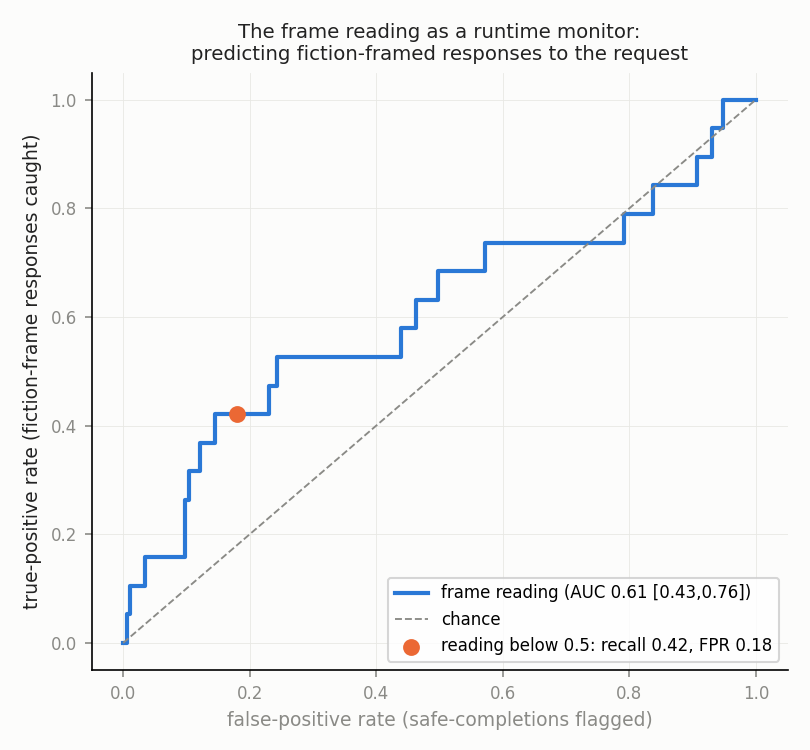
\includegraphics[width=\linewidth]{fig_s11_monitor_roc.png}
\caption{The frame reading as a standalone monitor, an exploratory check added after the analysis freeze. Receiver operating characteristic for predicting fiction-framed responses to the request (responses that take up the fictional frame rather than safe-completing) from the calibrated-site reading alone: the true-positive rate (fiction-framed responses caught) against the false-positive rate (safe-completions flagged). The AUC is 0.61 [0.43, 0.76], with a 95\% interval clustered by scene family (\S2.3), compatible with chance (dashed line). The marked point is one threshold, with its recall and false-positive rate.}\label{fig:fig_s11_monitor_roc}
\end{figure}
\FloatBarrier

\section{Limitations and future work}

\textbf{One model, stated plainly.} Everything here is measured in one
20-billion-parameter mixture-of-experts model, with deterministic decoding. Each
dynamics claim is made at one calibrated site and layer per task — single rows of a
depth progression in which crossing timescales vary systematically (\S3.2); no
single layer is a sufficient readout of the model's state, and behavior is produced
downstream of all of them. Within the
study, replication is internal: two task contrasts, three carriers plus a replicate, two
measurement sites, twelve scene families per class per task. That inventory also records what did \emph{not}
replicate cleanly: the
real$\rightarrow$fictional remnant is suggestive only once reference uncertainty is propagated; the
letter-site asymmetry rests on four runs per direction; 48\% of fiction/real runs are
indeterminate under per-run model selection; and our pre-stated prediction about the
ordering of crossing times across layers held in one task and failed in the other.
Cross-task patterns — the task with the wider endpoint separation also shows the larger
remnant gaps; anchored versus distributed contrast structure — are n = 2 observations,
hypotheses rather than findings.

\textbf{The named open question.} Whether the remnant — and the dwelling within the
unresolved zone — are permanent or merely slower than twenty sentences: in the terms of
\S4, whether the dwelling is a pun rather than a long garden path — is decidable by
extending the post-shift horizon (extended-tail runs) and by shifting evidence back to
the original class (A$\rightarrow$B$\rightarrow$A runs, measuring what remains of the second frame). Both are
designed and costed; neither has run.

\textbf{Further deferred work,} in rough order of leverage:

\begin{itemize}
\item Replicating the fiction/real headline quantities at the ' write' site, where the
framing contrast reads most strongly (the existing recordings suffice).
\item Expanding the letter-site families.
\item Calibration sets from a third, unrelated class, to identify what the accumulation
offset contains.
\item Monitor construction (multi-site, marker-augmented, depth-aware) against the
chance-compatible single-site baseline reported above.
\item Causal localization of where safeguard behavior reads in the stack: patching shallow
versus mid-stack states during generation — the decisive test for \S4's three
candidate accounts.
\item A planned suite of harder context manipulations — colliding frames, mutating them
mid-context, deliberately incoherent contexts — where genuine off-distribution
excursions are most likely, our clean block-shifts being the tamest possible case.
\end{itemize}

The analyses reported here were frozen before drafting; the post-freeze additions are
logged as such in Appendix B.


\section*{Back matter (assembly spec --- materialized at final build)}
\emph{Review-draft note: the sections below are the assembly specification; the final build replaces them with the referenced frozen content.}


\subsection*{Acknowledgments}
[Agreed AI-assistance line — exact text from Andrew/chat side, placeholder.] Personal
acknowledgments: Andrew adds.

\subsection*{Related work (arXiv default: standalone section, drafted from handoff \S6 anchors)}
Probing validity: Alain \& Bengio; Hewitt \& Liang (control tasks — our D5 + label-shuffle
audits presented as the selectivity answer); Belinkov survey. Directions \& steering:
Marks \& Tegmark (also the mass-mean/diff-of-means probing precedent for \S2.2's
axis choice); Arditi et al. (refusal direction — nearest cousin of the fiction/real
behavior link). In-context dynamics: Xie et al. (ICL as implicit Bayesian inference —
the standing theory our integrator null speaks to); Hendel; Todd (function vectors);
Olsson et al. (induction heads). Safety: many-shot jailbreaking; Crescendo-style
multi-turn escalation. Psycholinguistics: Christianson \& Ferreira; Slattery et al.; van
Schijndel \& Linzen. Verbalized uncertainty \& ambiguity (grounds the intro's scoped
claim): Kadavath et al.; Lin et al. (verbalized confidence); Xiong et al. (calibration
of verbalized confidence); Liu et al. (ambiguity modeling). Internal encoding vs
expression (grounds Discussion's ``represented but not consulted''): Azaria \& Mitchell
(internal state predicts truthfulness); Orgad et al. (models encode more than they
express). Long-context artifacts: attention sinks (the ``is the offset positional?''
question; midpoint referencing makes our findings robust either way). Dynamics: Sussillo
\& Barak; Kelso; Rabinovich et al. Motivating
case (intro + discussion): Raine v. OpenAI, Cal. Super. Ct. (S.F.), filed
2025-08-26; contemporaneous reporting (CNN 2025-08-26; NBC News; TechCrunch
2025-11-26 on OpenAI's answer denying causation). Contested litigation — the paper
characterizes only what the filing and reporting describe. Model provenance (the
intro's ``trained safeguard''): gpt-oss model card, safety training documented.

\subsection*{Appendix A — Corrections affecting reported values}
One line each for the corrections that changed numbers as printed: the real$\rightarrow$fictional
remnant interval widening to include zero under reference resampling; the trimmed
within-stream means; the per-run crossing-time medians; the recency-parameter memory
figures. The complete corrections record is in the repository.

\subsection*{Appendix B — QA and reproducibility}
Regeneration audit summary (bit-identical axes; 23-script diff green; seeded bootstraps
exact); 9/9 fixture suite; sign/boundary/join/shuffle audits; the four logged post-freeze
additions (s12 response counts, 0/96; s11 monitor ROC, AUC 0.61 [0.43,0.76]; s13
per-layer collapse panels; s14 exploratory per-layer behavior association — both
computed from frozen captures via the committed cache); repository
pointer + regeneration instructions. Terminology map for repository readers: the paper's
\emph{remnant} is the repository's ``residual''; the dwelling within the unresolved zone is the
repository's ``park''; \emph{accumulation offset} is ``accumulation drift''; \emph{tasks} are the
repository's ``probes''/``probe arms''; corpus directories D3/D4/D5/D6 are the transition,
no-shift, minimal-pair, and mixture-sweep corpora; the repository's ``K=1'' label names an
analysis convention for a routing track this study dropped.

\subsection*{Appendix C — Supplementary figures}
figures/other/ (12): fr fit gallery, fr D6 loop, tank secondary heatmap, matched-k panel
is MAIN (\texttt{fig\_s9\_behavior\_matchedk}) — supplement gets: raw + midref heatmap generations
(the instrument story's ``before'' pictures), prelexical\_L4, occupancy\_bands\_L4,
jumpiness, norm\_vs\_alignment, calibration\_layers, plus \texttt{fig\_s11\_monitor\_roc}. \texttt{fig\_s13\_collapse\_layers} is MAIN (cited
in \S3.2's depth paragraph; committed script s13\_collapse\_by\_layer.py).

\end{document}
